\section*{Supplements}
\subsection*{\inlineprogram{CellSegmentationEvaluation}- Parameters}
\begin{itemize}
\centering
    \item[NC] Number of cells per 100\unit{\micro\square\meter}
    \item[FFC] Fraction of image foreground occupied by cells
    \item[1-FBC] Fraction of image background occupied by cells
    \item[FCF] Fraction of cell mask in coeground
    \item[FMCN] Fraction of match between cells and nuclei
    \item[1/(ACVE+1)] Average CV of foreground pixels outside the cells
    \item[FPCF] Fraction of first PC of foreground pixels outside of cells
    \item[1/(ACVC+1)] Average of weighted average CV of cell type intensities over 1-10 clusters
    \item[FPCC] Average of weighted average fraction of the first PC of cell type intensities over 1-10 clusters
    \item[AS] Average Silhouette score of clustering over 2-10 clusters
    \item[1/(ln(CSSD)+1)] Standard deviation of cell size
\end{itemize}
\subsection*{Directory-Structure}
\begin{figure}[ht]
    \small
    \dirtree{%
        .1 \textless sample name\textgreater.
        .2 processed.
        .3 \textless section\textgreater.
        .4 boundaries.
        .5 cell\us relative.parquet.
        .5 nucleus\us relative.parquet.
        .4 morphology.
        .5 focus.
        .6 focus.ome.tif.
        .6 quartered.
        .7 q0\%c.ome.tif.
        .5 multi\us layer.
        .6 morphology.ome.tif.
        .6 quartered.
        .7 q0\%c.ome.tif.
        .5 single\us layer.
        .6 layer0\%L.
        .7 morphology.tif.
        .7 quatered.
        .8 q0\%c.tif.
        .4 transcripts.
        .5 relative.csv.
        .5 relative.parquet.
        .3 marked\us regions-of-interest.tif.
        .3 sections\us px.json.
        .2 results.
        .3 \textless method\textgreater.
        .4 evaluation.
        .5 \textless section\textgreater.
        .6 layer.
        .7 DC-TOOLS.csv.
        .7 false\us negatives.csv.
        .7 results.csv.
        .7 split\us merges.csv.
        .4 output.
        .5 \textless section\textgreater.
        .6 \textless ...\textgreater.
        .2 run.
        .3 jobs.
        .4 \textless method\textgreater.sh.
        .3 logs.
        .4 \textless method\textgreater\us \%N\us \%j.err.
        .4 \textless method\textgreater\us \%N\us \%j.out.
    }
    \caption{Final structure of the directories after a run of the custom pipeline.}
    \label{fig:directory structure}
\end{figure}

\subsection*{Segmentations}
\begin{figure*}[t!]
    \centering
    \begin{subfigure}[t]{0.5\textwidth}
        \centering
        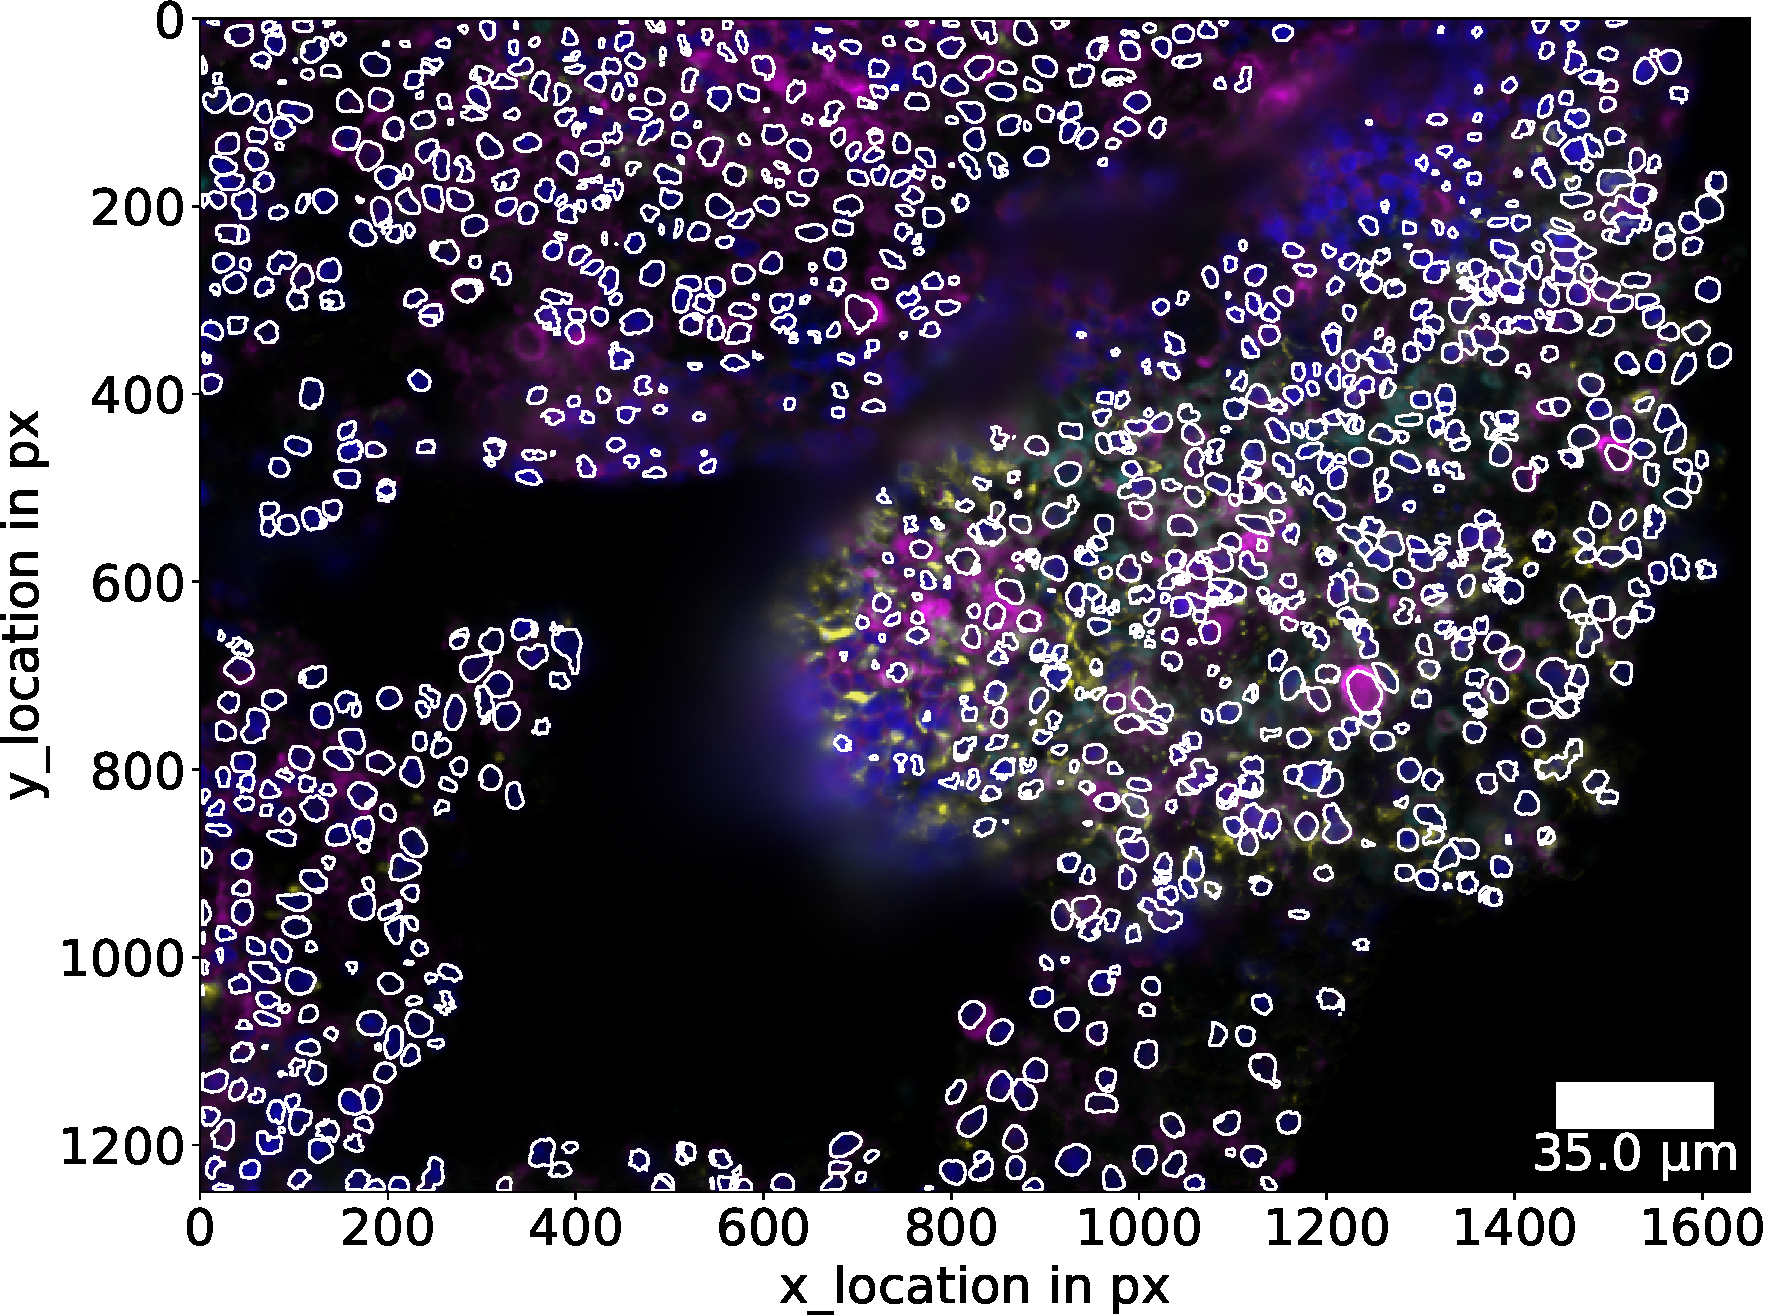
\includegraphics[width=\linewidth]{Images/SI/outlines/outline_cpsam_polygons_focus.pdf}
        \caption{Masks by \textsc{CPSAM}; Input: \inlinepath{morphology-focus}, all channels.}
        \label{fig:Overlay_cpsam}
    \end{subfigure}%
    ~ 
    \begin{subfigure}[t]{0.5\textwidth}
        \centering
        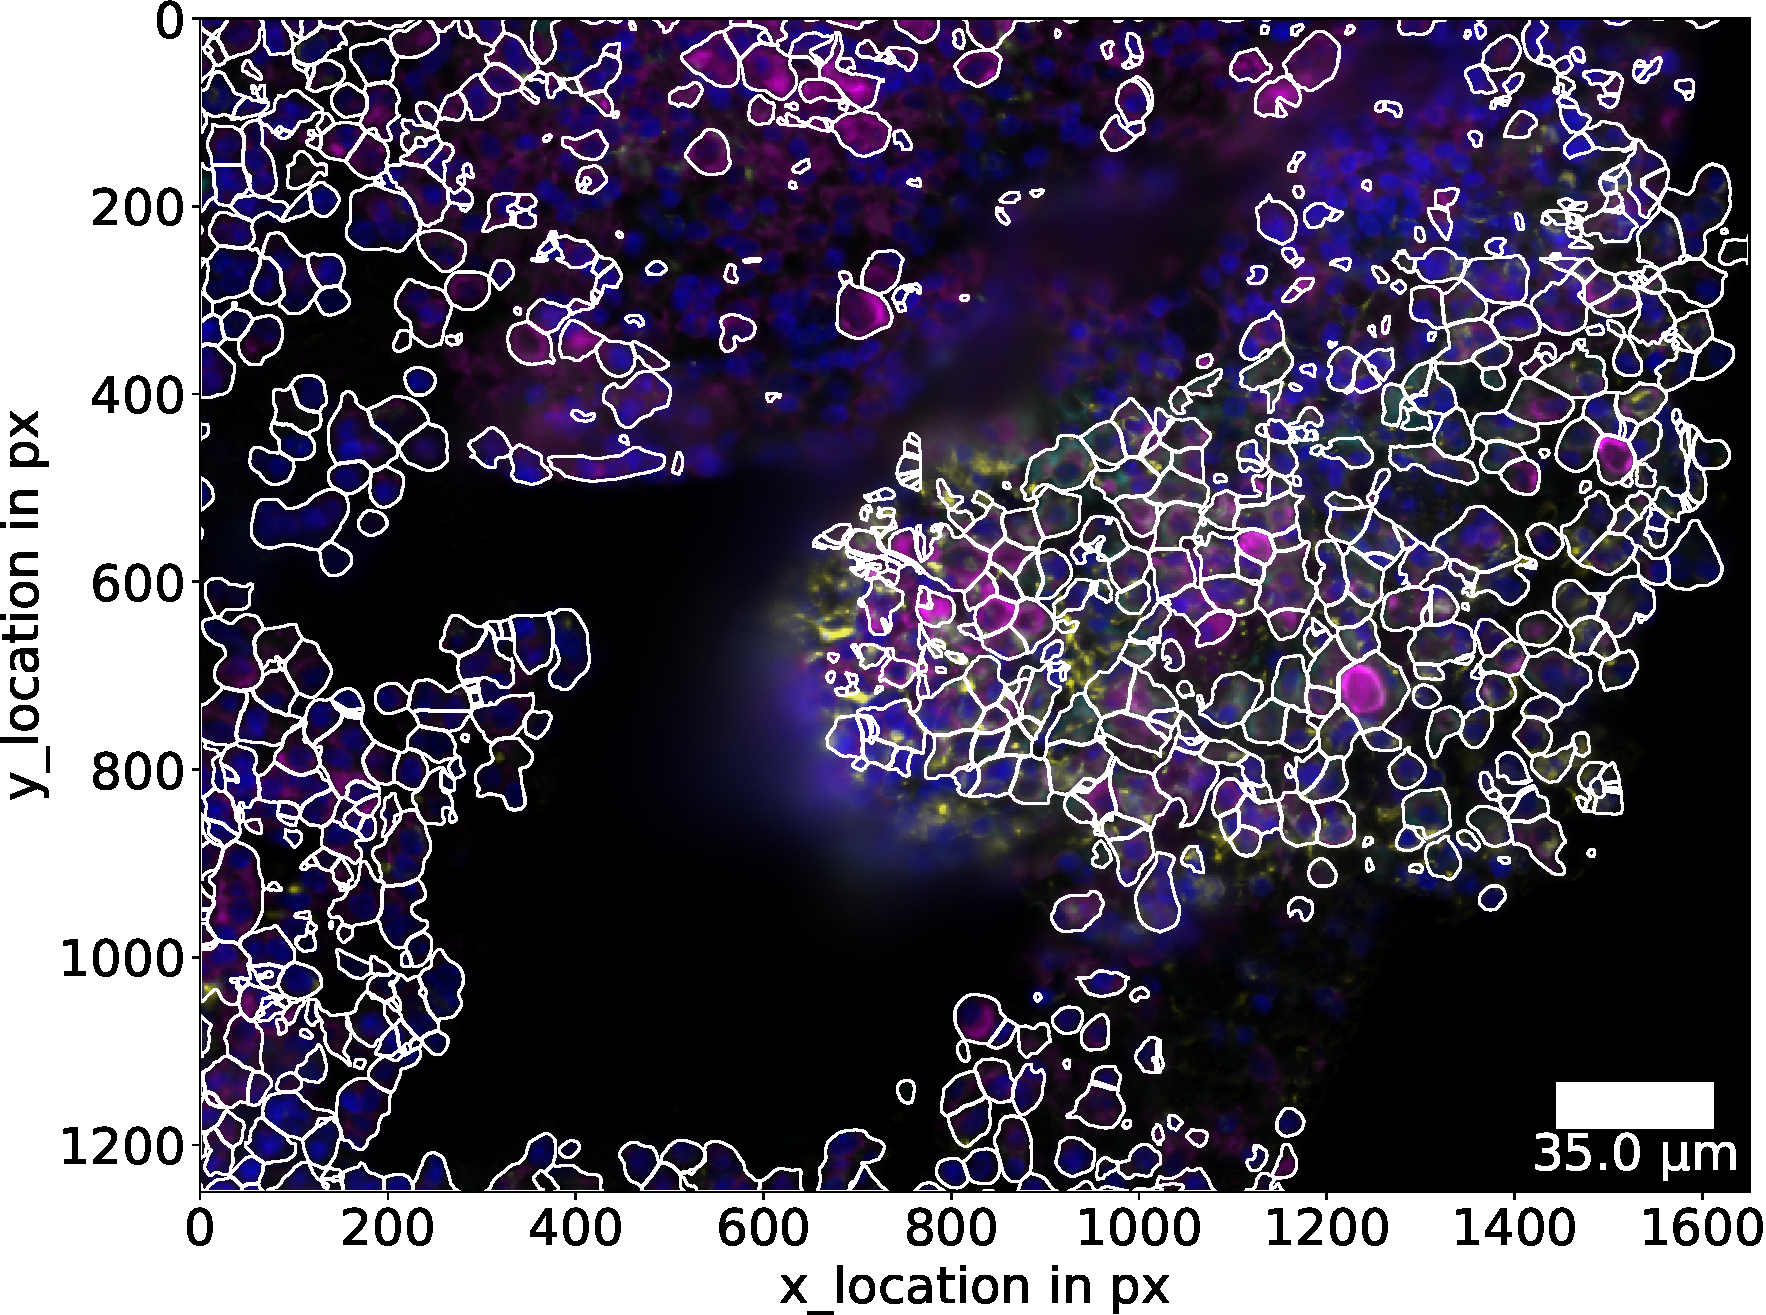
\includegraphics[width=\linewidth]{Images/SI/outlines/outline_dinocell_polygonsn.pdf}
        \caption{Masks by \textsc{DINOCell}; Input: \inlinepath{morphology-focus}, all channels.}
        \label{fig:Overlay_dino}
    \end{subfigure}%
    \vskip\baselineskip
    \begin{subfigure}[t]{0.5\textwidth}
        \centering
        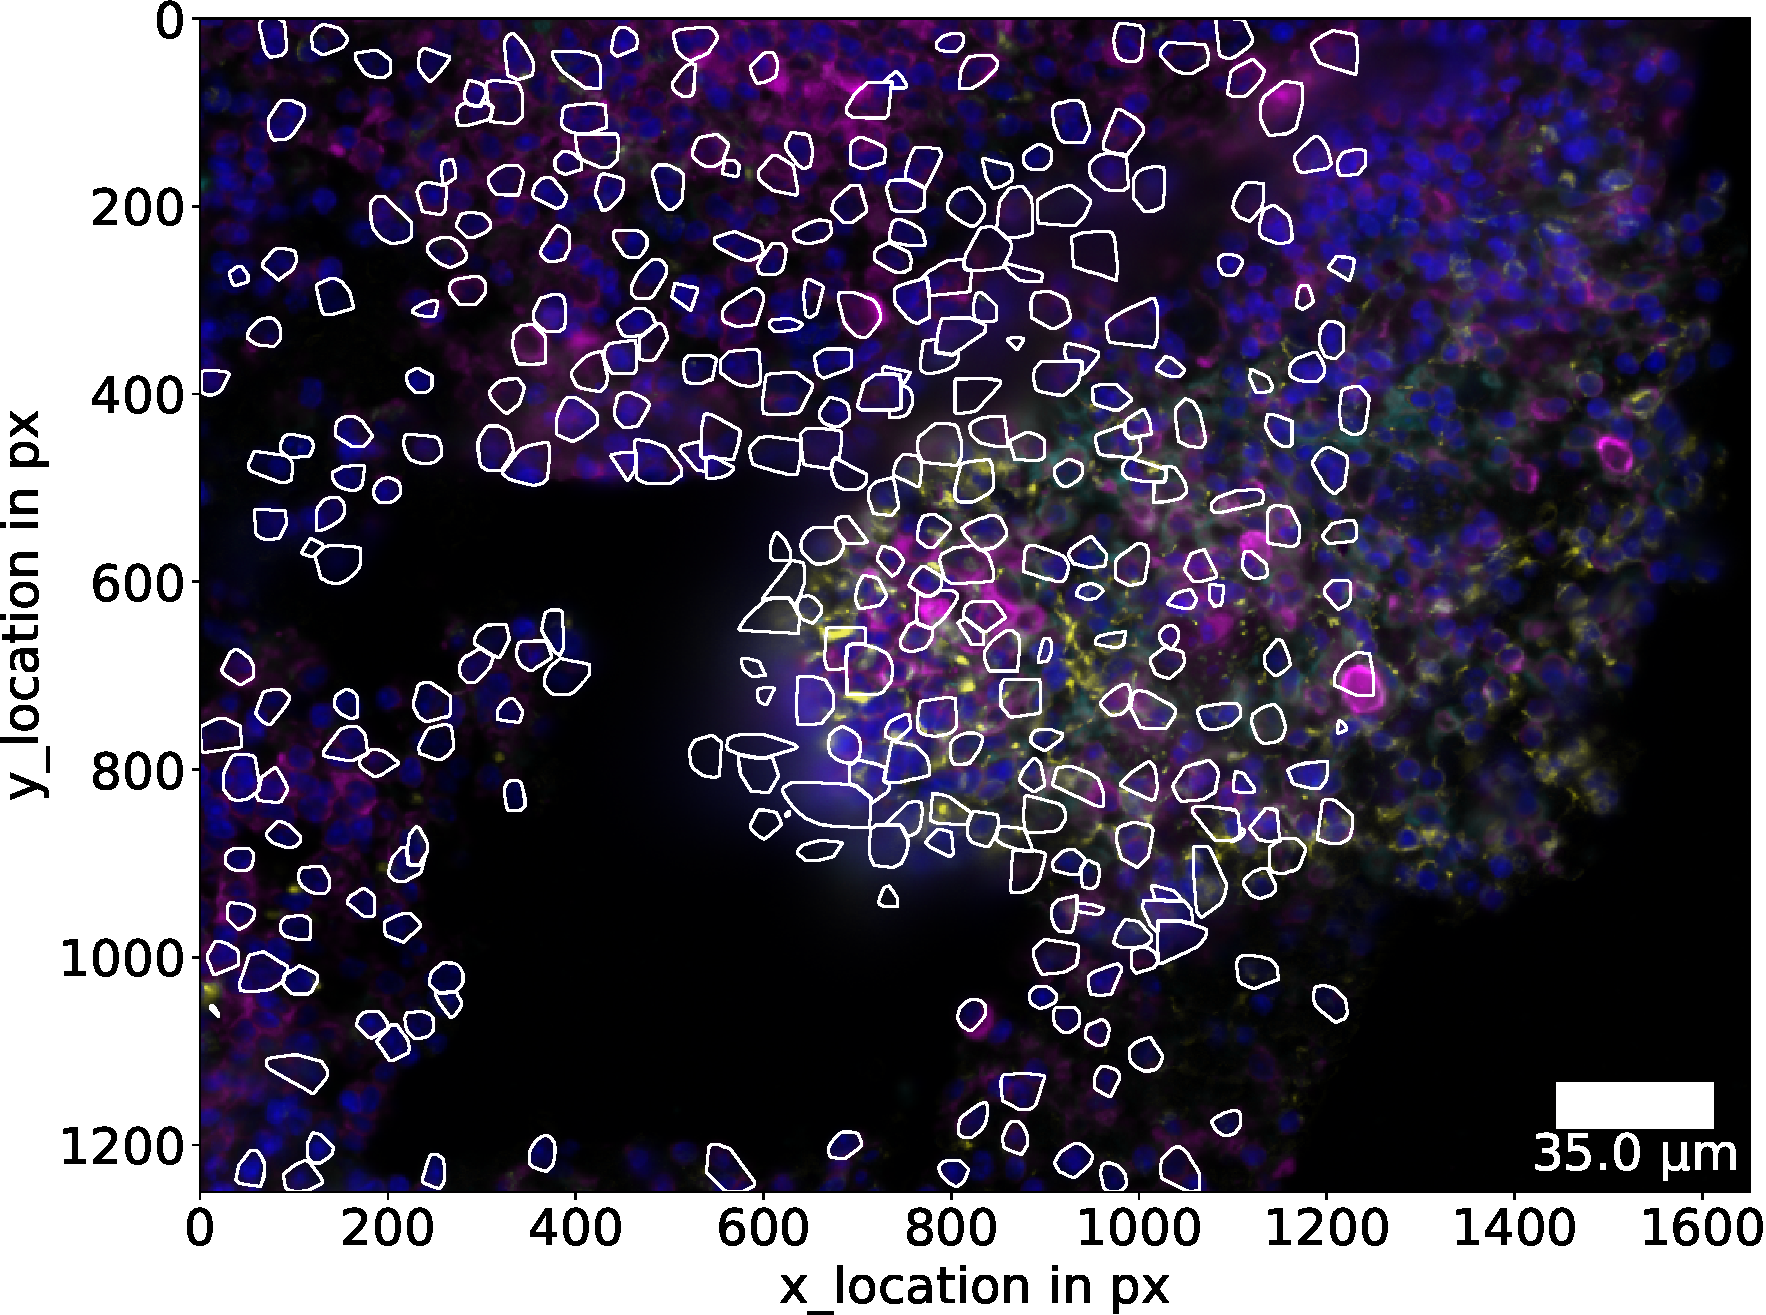
\includegraphics[width=\linewidth]{Images/SI/outlines/outline_dissect_polygonsn.pdf}
        \caption{Masks by \textsc{DISSECT}; Input: \inlinepath{morphology-focus}, all channels, and \inlinepath{transcripts}, located in the section and relative to its origin.}
        \label{fig:Overlay_dissect}
    \end{subfigure}%
    ~
    \begin{subfigure}[t]{0.5\textwidth}
        \centering
        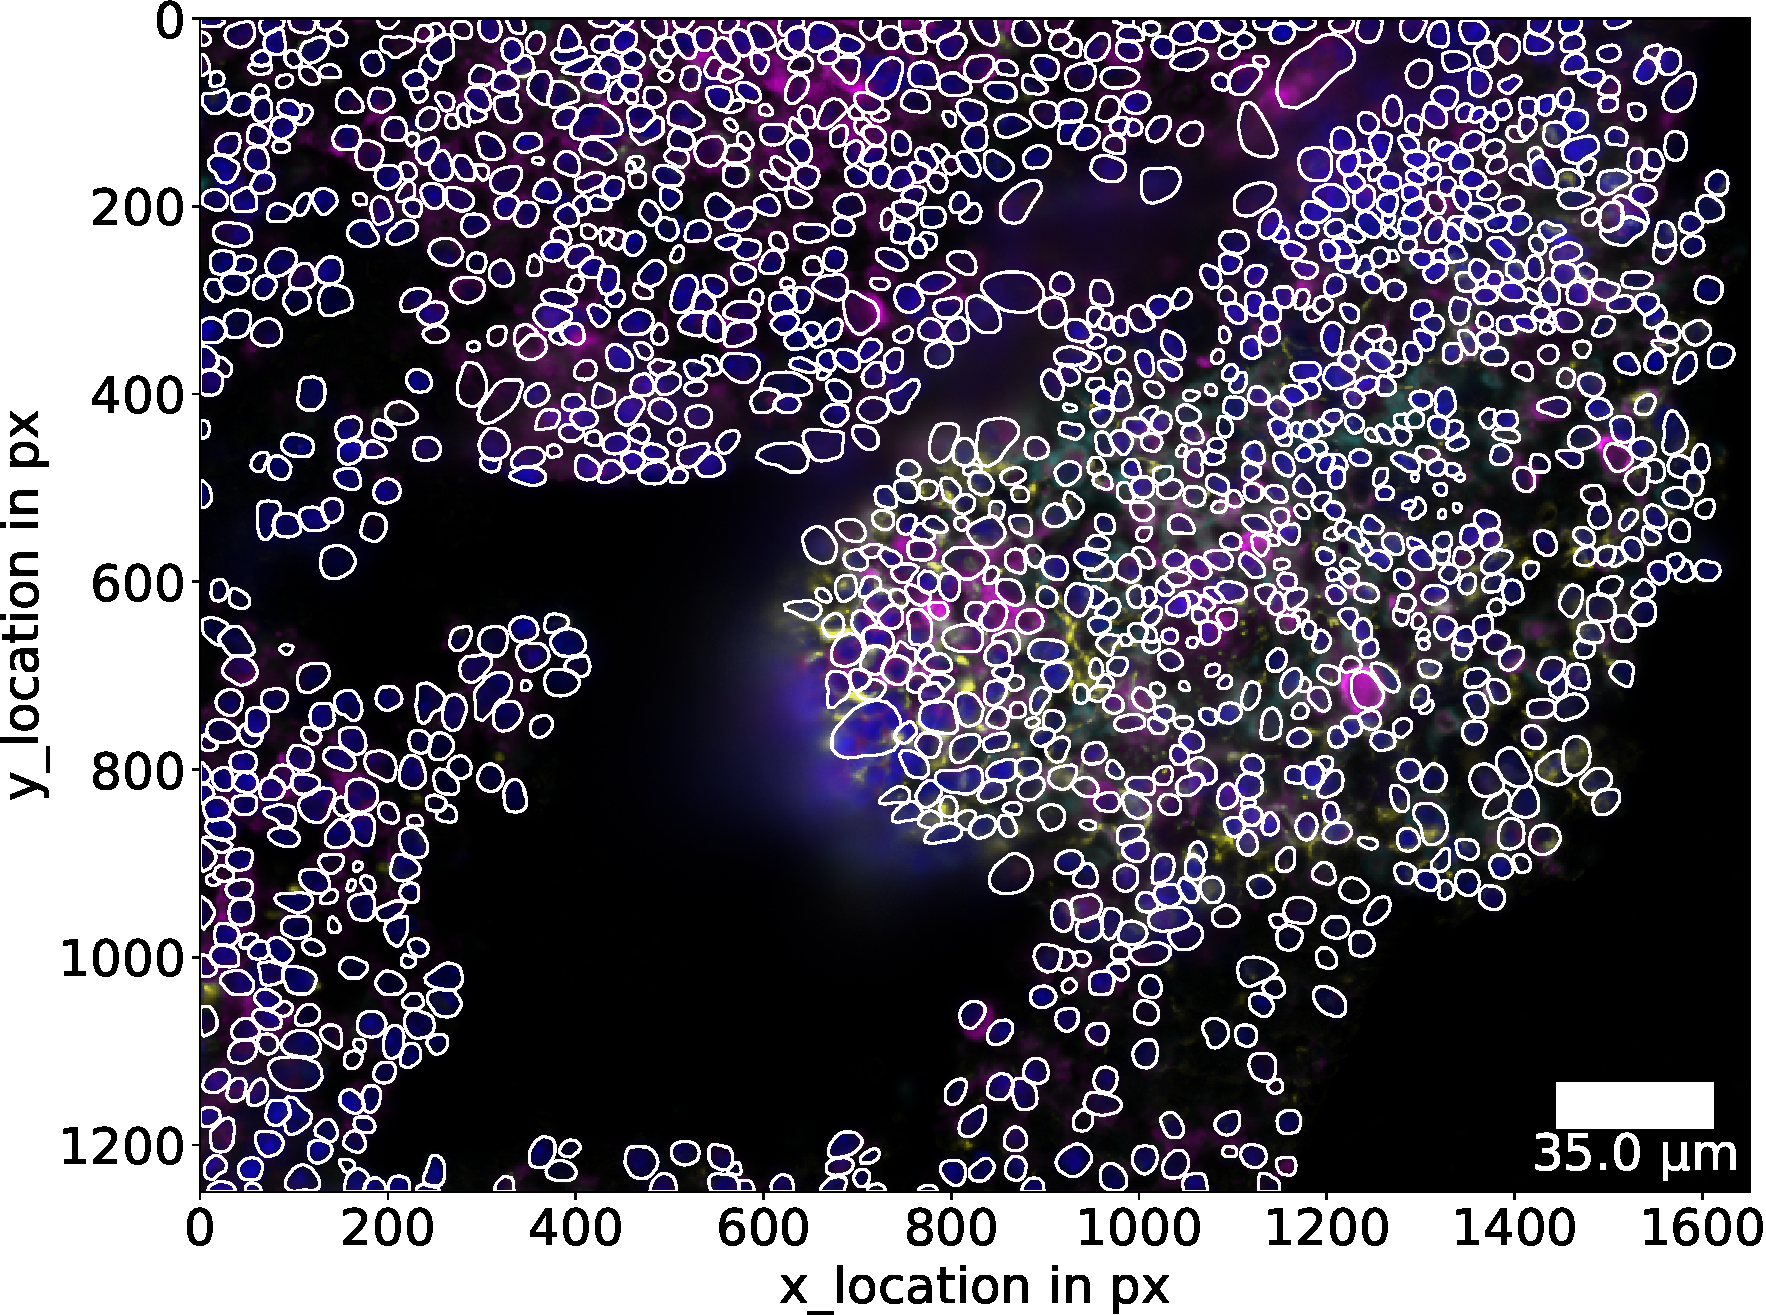
\includegraphics[width=\linewidth]{Images/SI/outlines/outline_stardist_polygons_focus.pdf}
        \caption{Masks by \textsc{StarDist}; Input: \inlinepath{morphology-focus}, DAPI channel.}
        \label{fig:Overlay_stardist}
    \end{subfigure}%
    \caption{Outlines of the predicted masks (white), overlayed on top of the \inlinepath{morphology-focus} image (blue: DAPI; cyan: ATP1A1/CD45/E-Cadherin; magenta: 18s rRNA; yellow: alphaSMA/Vimentin).}
    \label{fig:Outlines_0}
\end{figure*}

\begin{figure*}[t!]
    \begin{subfigure}[t]{0.5\textwidth}
        \centering
        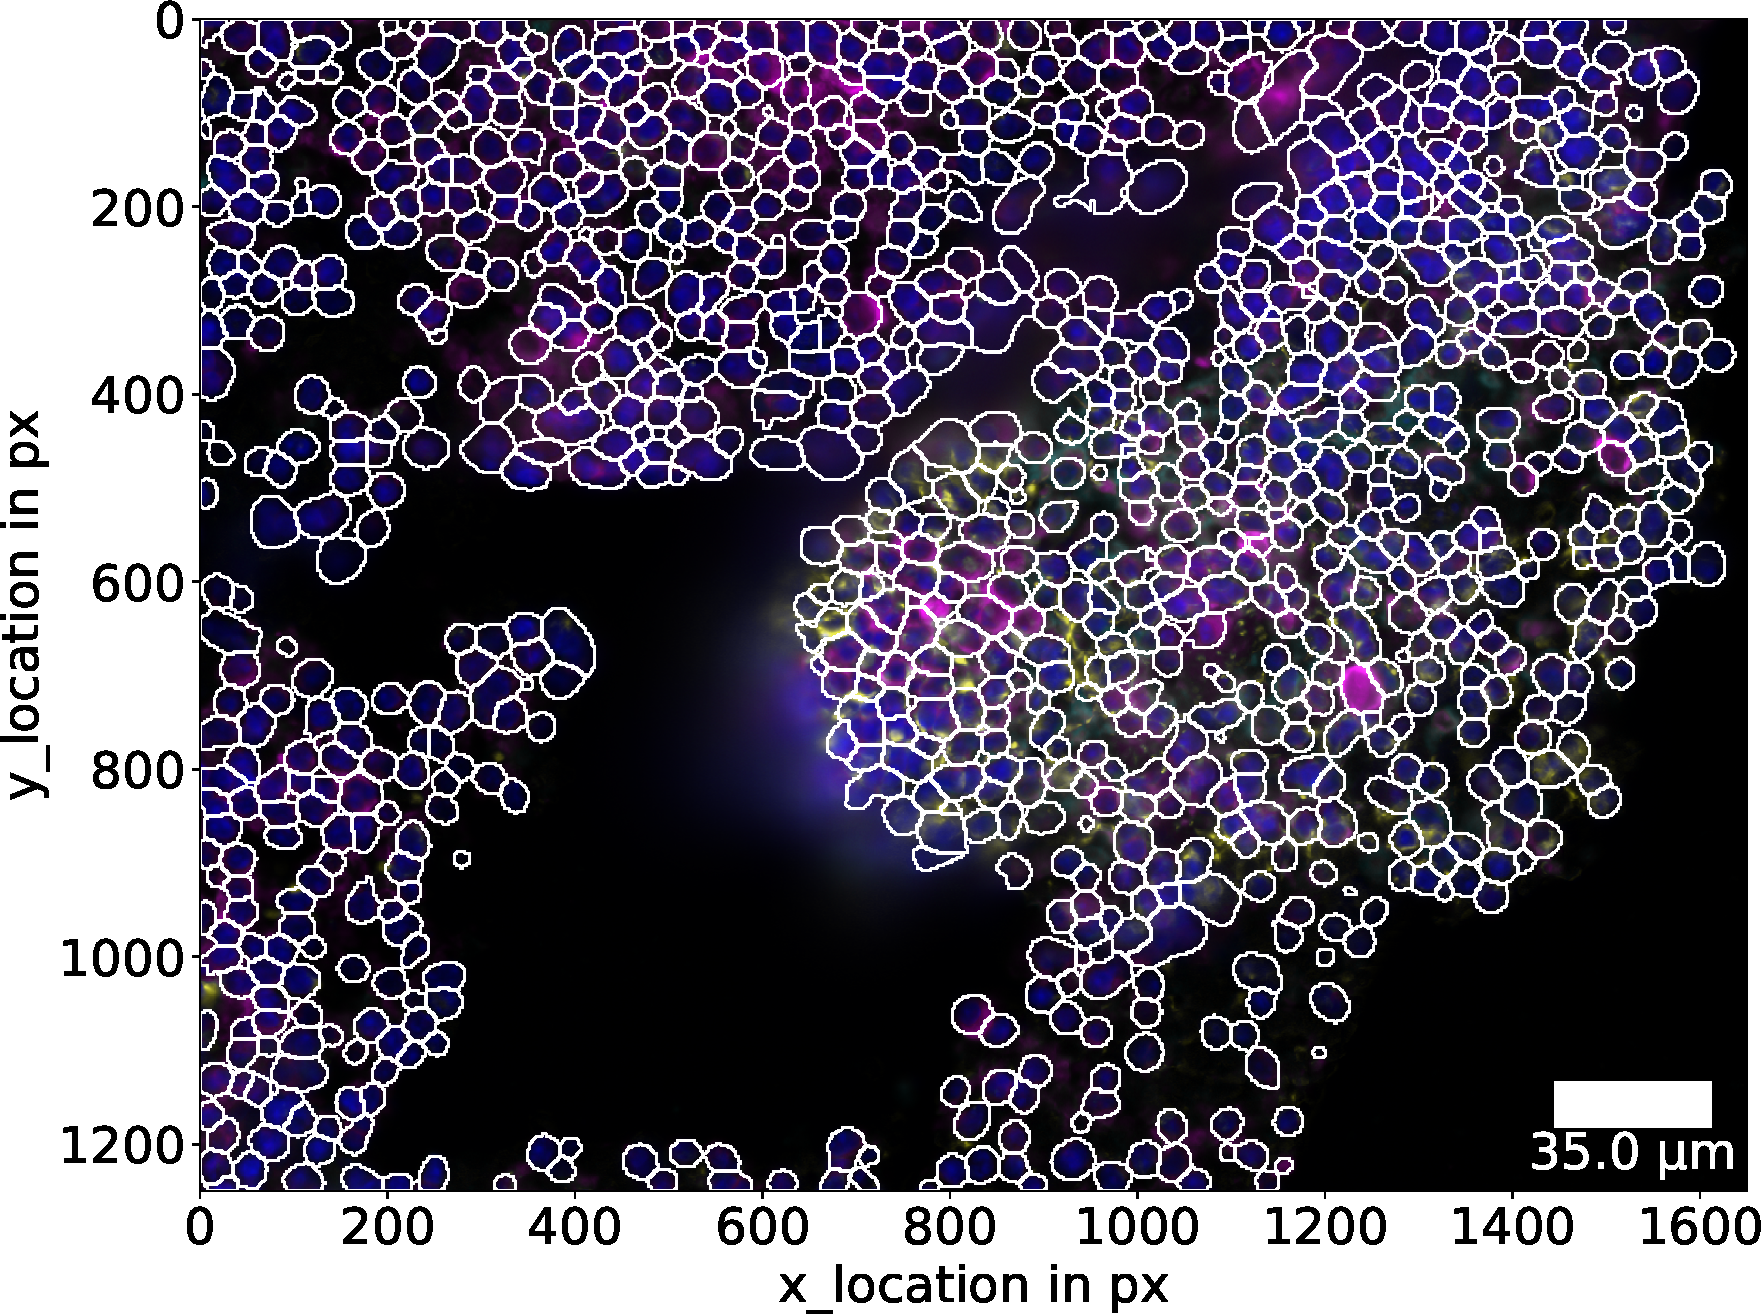
\includegraphics[width=\linewidth]{Images/SI/outlines/outline_mesmer_polygons_mt.pdf}
        \caption{Masks by \textsc{Mesmer}; Input: \inlinepath{morphology-focus}, DAPI channel with empty membrane/cytoplasm channel.}
        \label{fig:Overlay_mesmer_mt}
    \end{subfigure}%
    ~
    \begin{subfigure}[t]{0.5\textwidth}
        \centering
        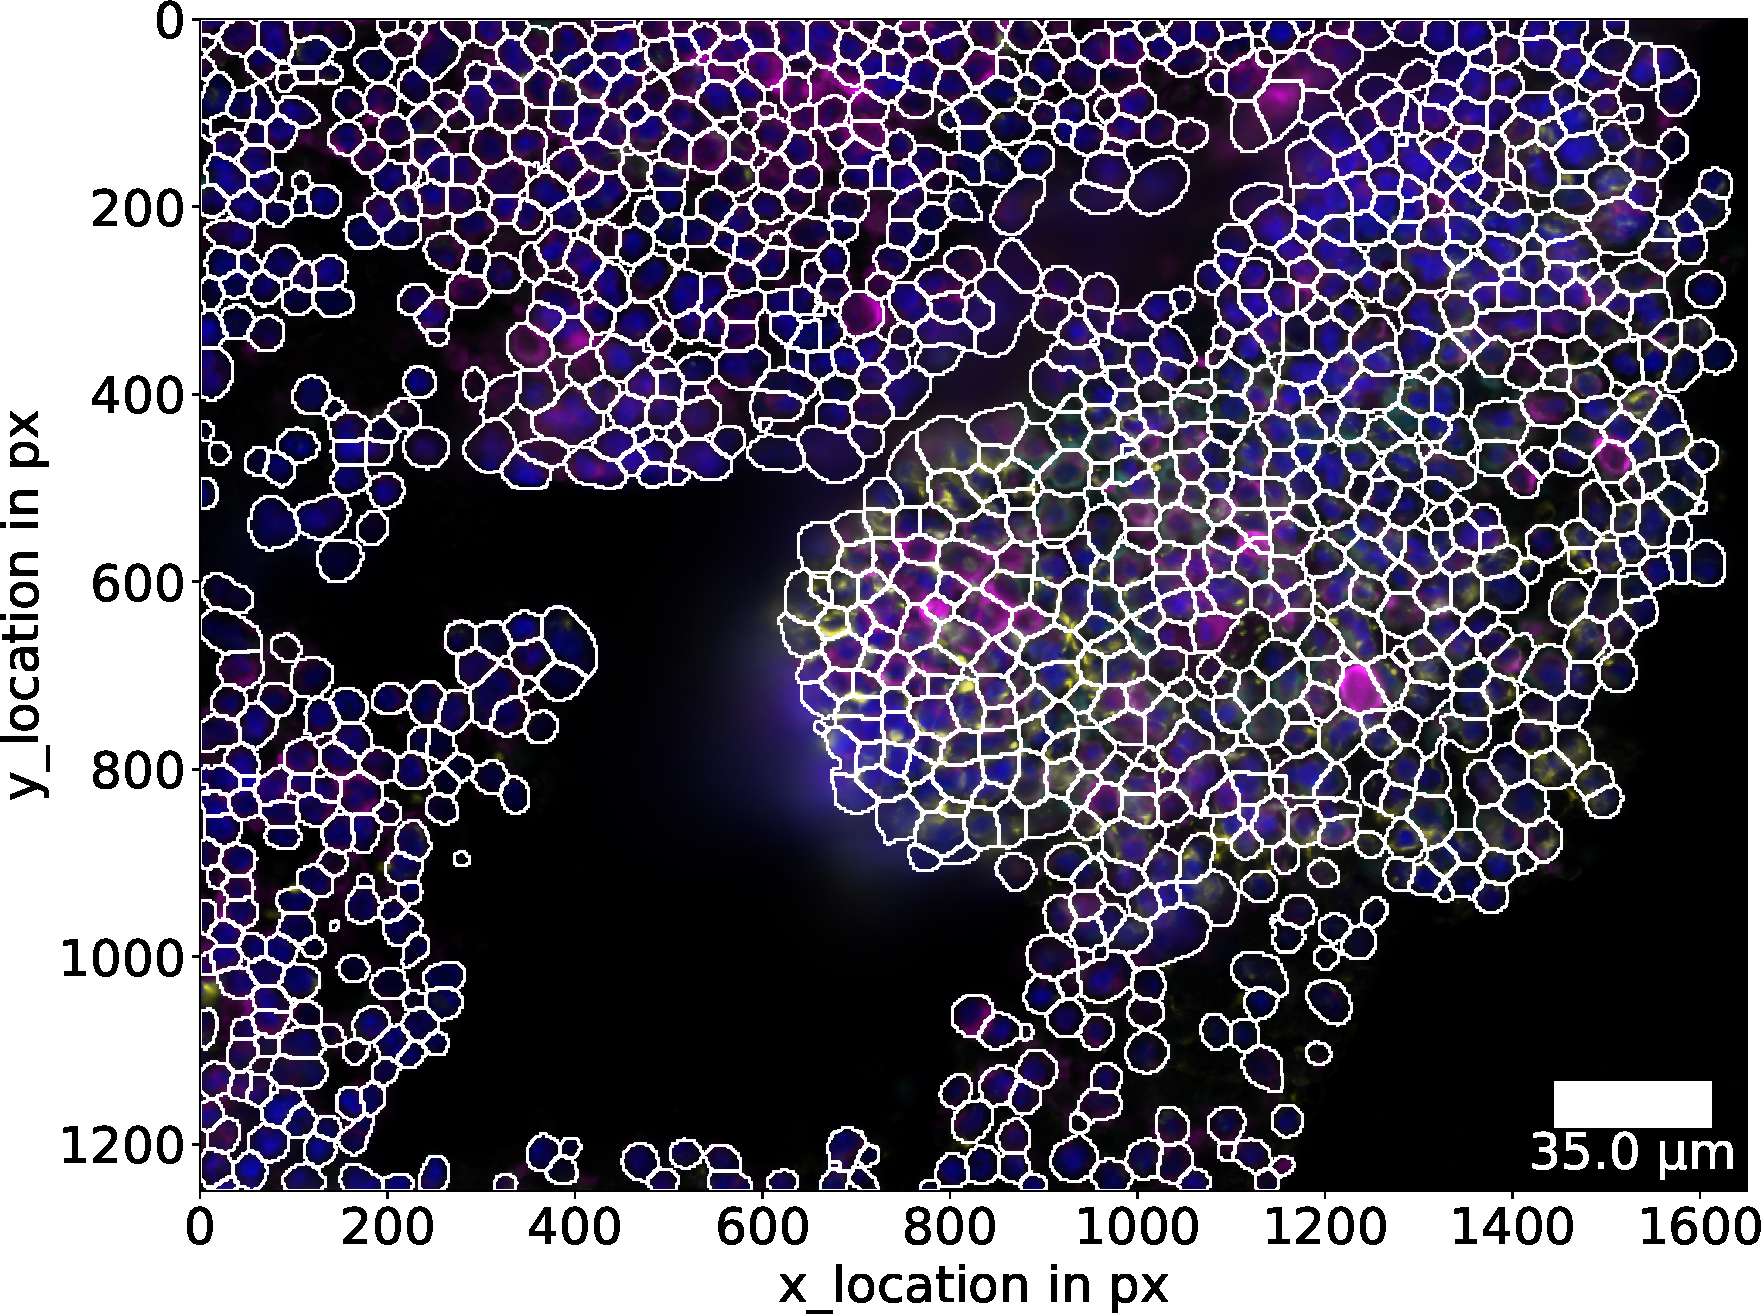
\includegraphics[width=\linewidth]{Images/SI/outlines/outline_mesmer_polygons_mem.pdf}
        \caption{Masks by \textsc{Mesmer}; Input: \inlinepath{morphology-focus}, DAPI channel and ATP1A1/CD45/E-Cadherin channel.}
        \label{fig:Overlay_mesmer_mem}
    \end{subfigure}%
    \vskip\baselineskip
    \begin{subfigure}[t]{0.5\textwidth}
        \centering
        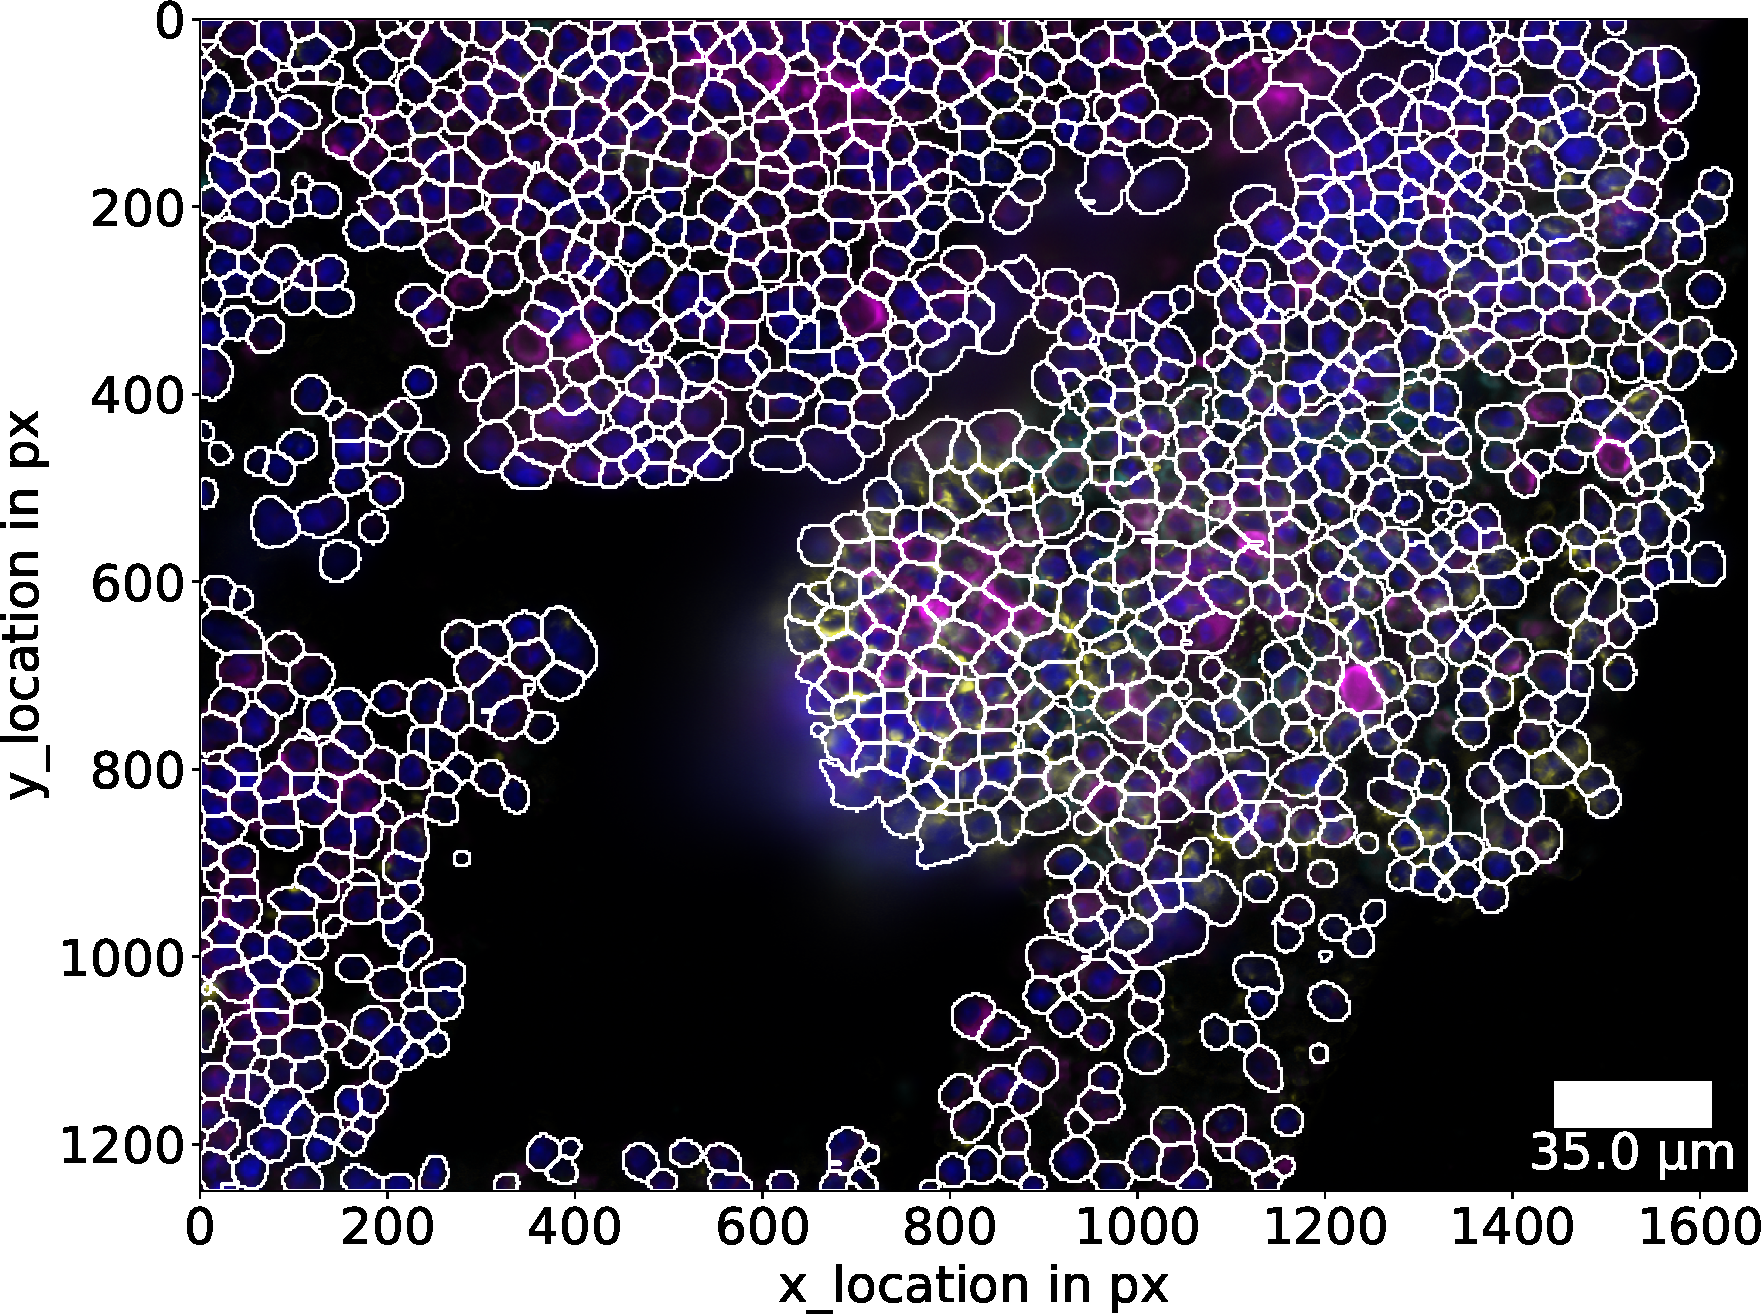
\includegraphics[width=\linewidth]{Images/SI/outlines/outline_mesmer_polygons_ribo.pdf}
        \caption{Masks by \textsc{Mesmer}; Input: \inlinepath{morphology-focus}, DAPI channel and 18s rRNA channel
        \label{fig:Overlay_mesmer_ribo}
    \end{subfigure}%
    ~
    \begin{subfigure}[t]{0.5\textwidth}
        \centering
        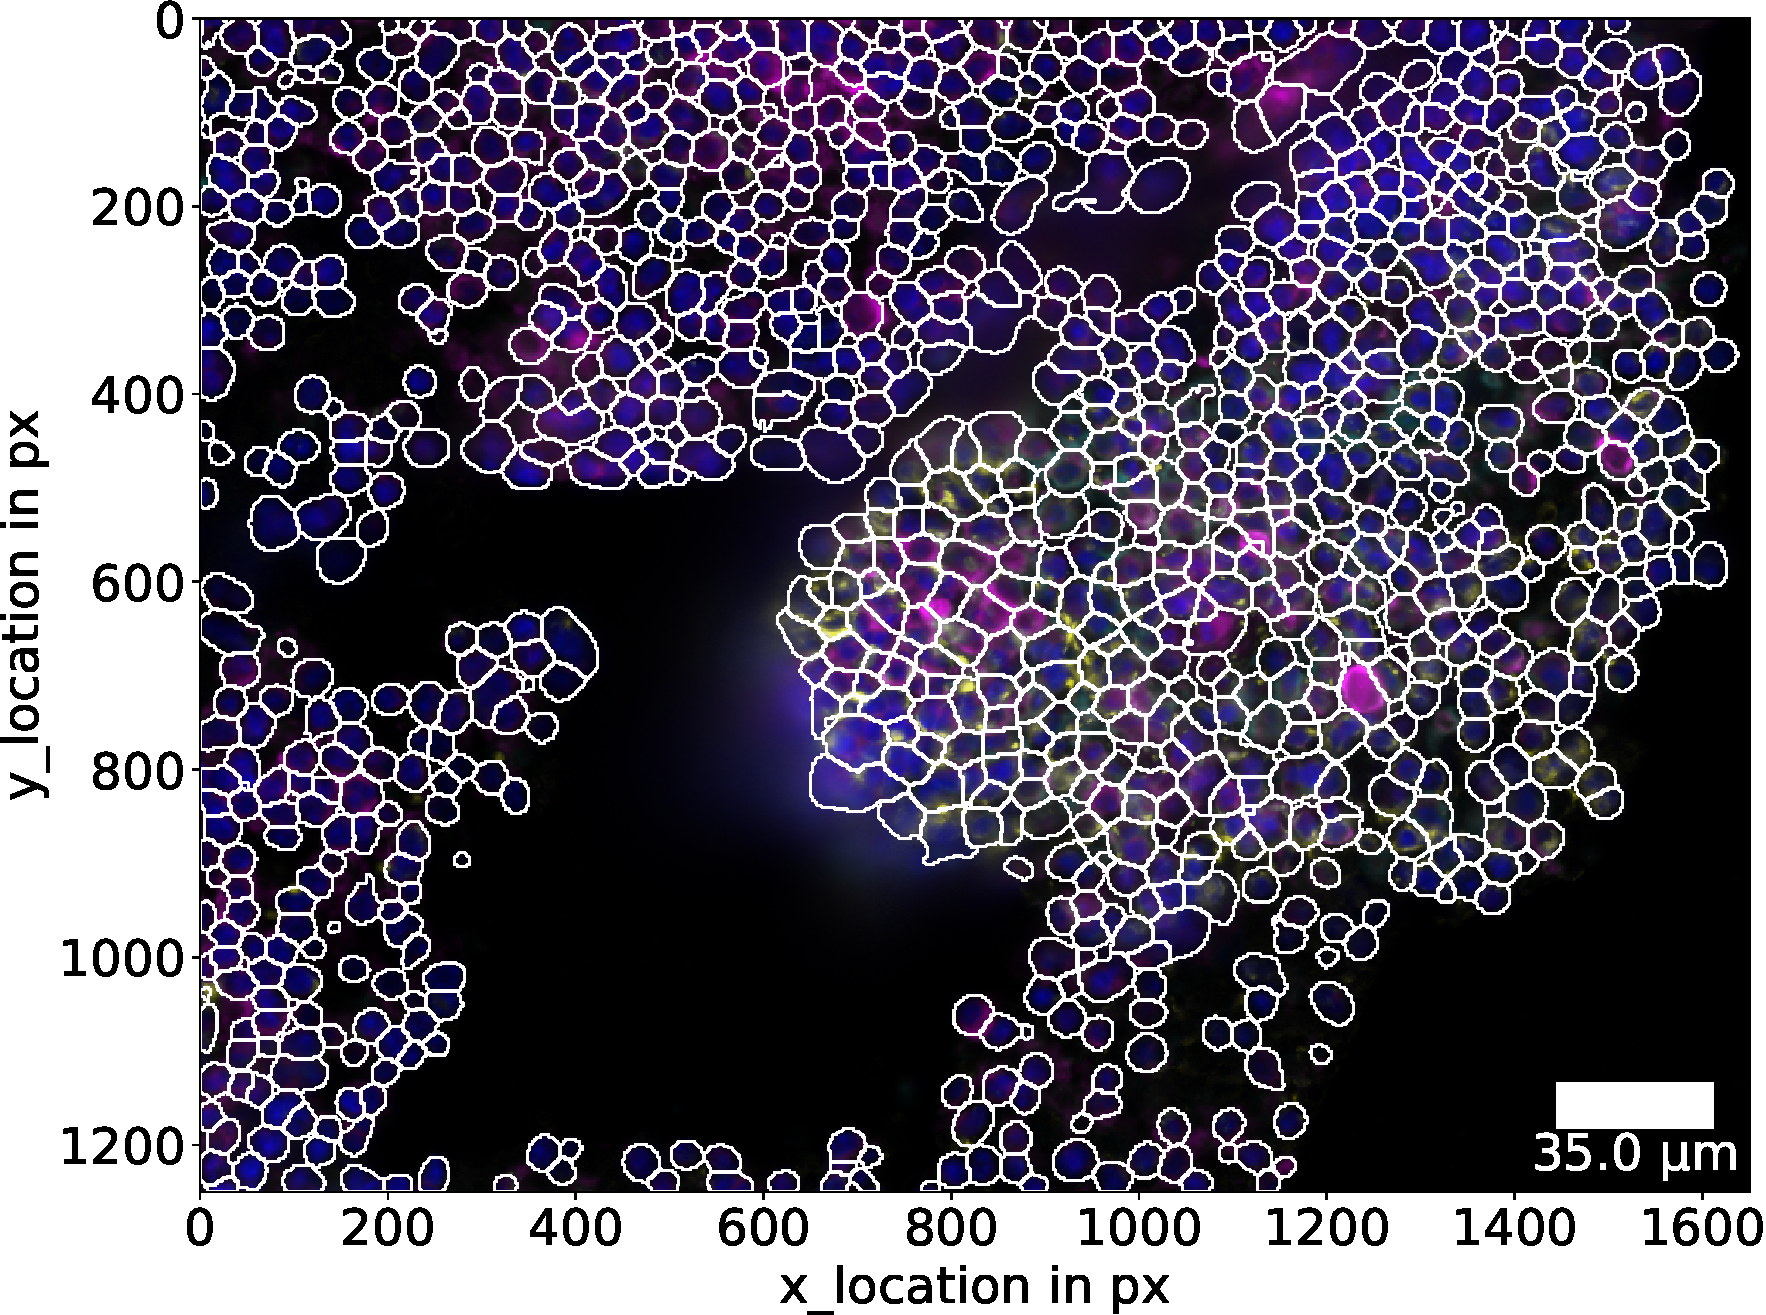
\includegraphics[width=\linewidth]{Images/SI/outlines/outline_mesmer_polygons_cyto.pdf}
        \caption{Masks by \textsc{Mesmer}; Input: \inlinepath{morphology-focus}, DAPI channel and alphaSMA/Vimentin channel.}
        \label{fig:Overlay_mesmer_cyto}
    \end{subfigure}%
    \caption{Outlines of the predicted masks (white), overlayed on top of the \inlinepath{morphology-focus} image (blue: DAPI; cyan: ATP1A1/CD45/E-Cadherin; magenta: 18s rRNA; yellow: alphaSMA/Vimentin).}
    \label{fig:Outlines_1}
\end{figure*}

\begin{figure*}[t!]
    \begin{subfigure}[t]{0.5\textwidth}
        \centering
        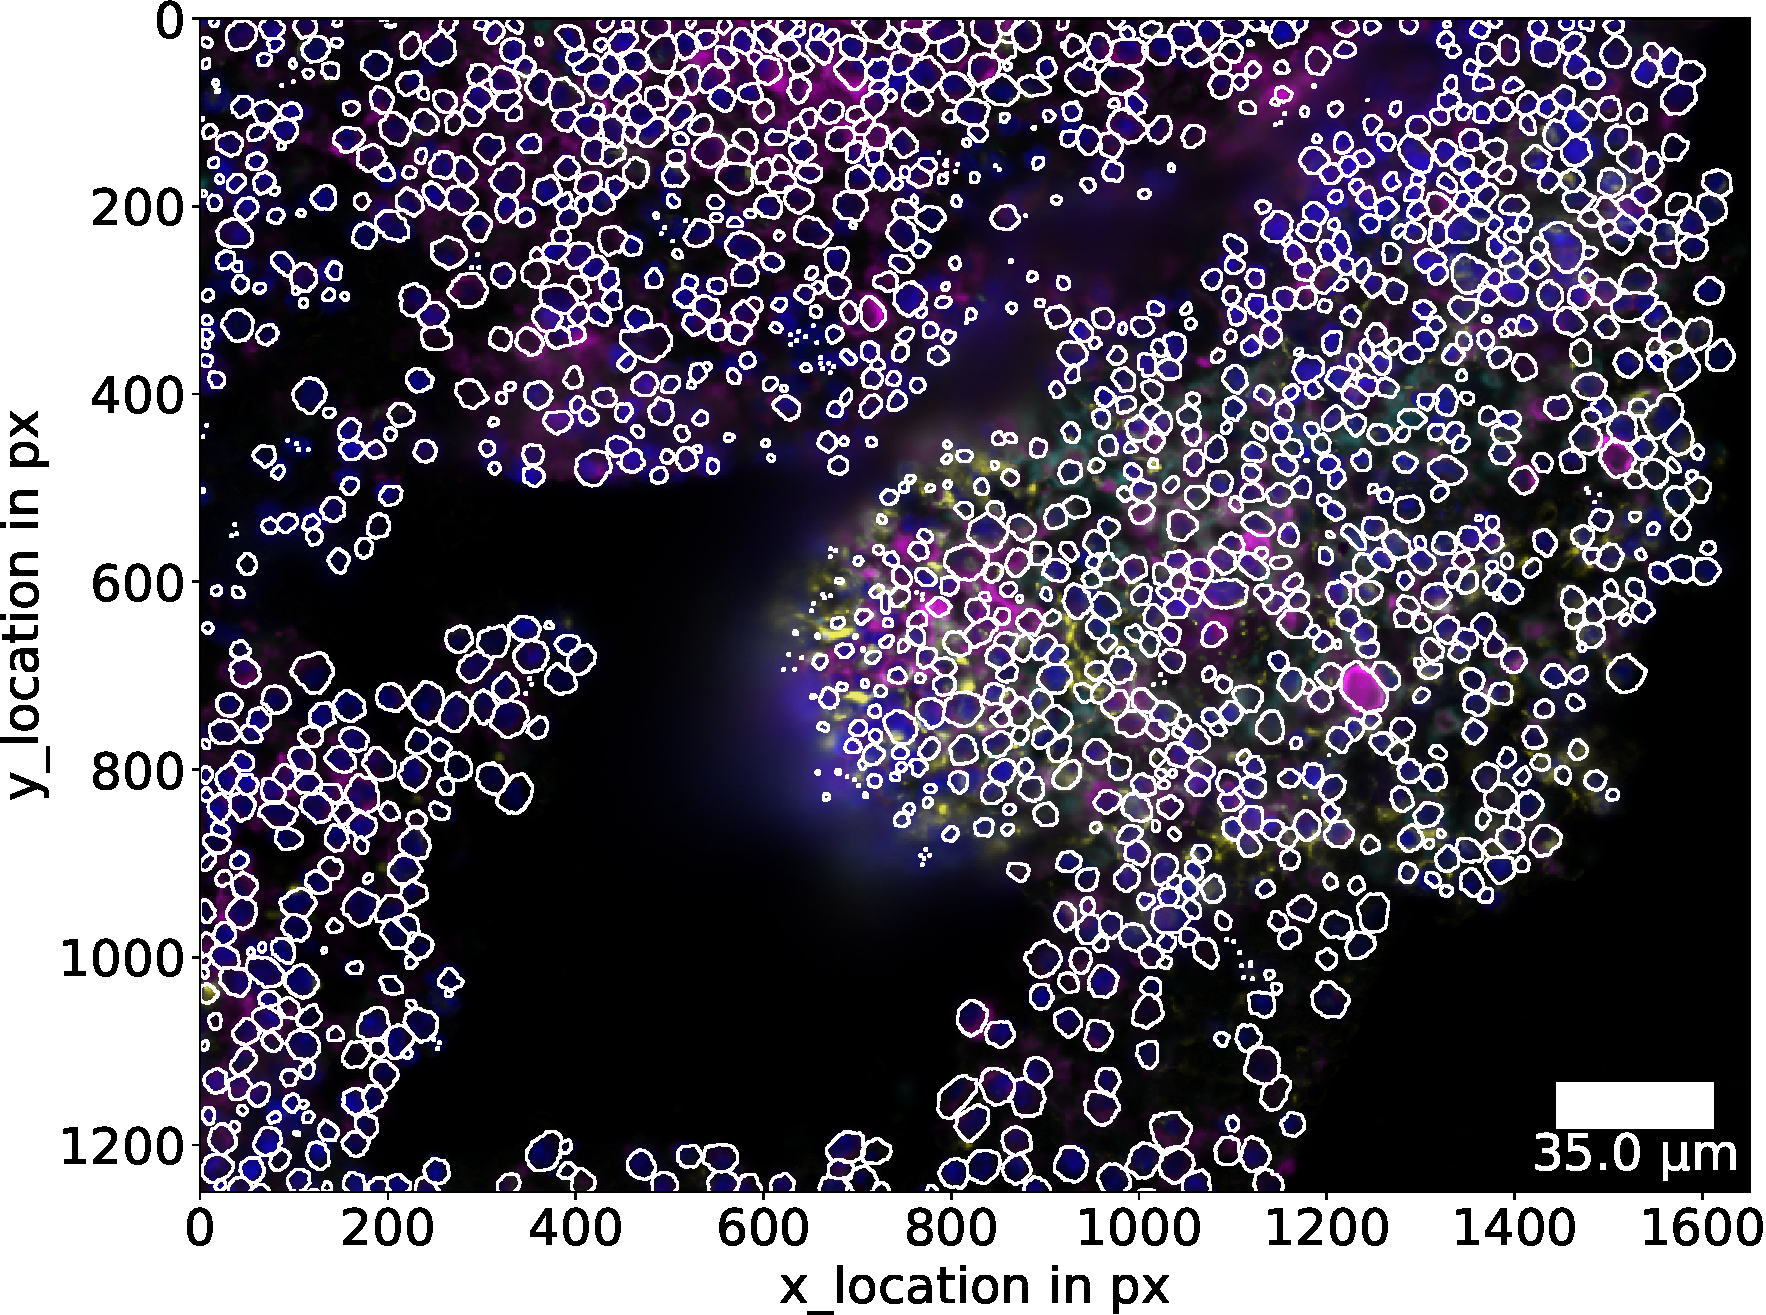
\includegraphics[width=\linewidth]{Images/SI/outlines/outline_proseg_cell-polygon-layers.geojson0.pdf}
        \caption{"Layer 0"-masks by \textsc{ProSeg}; Input: \inlinepath{transcripts}, located in the section and relative to its origin.}
        \label{fig:Overlay_proseg_0}
    \end{subfigure}%
    ~ 
    \begin{subfigure}[t]{0.5\textwidth}
        \centering
        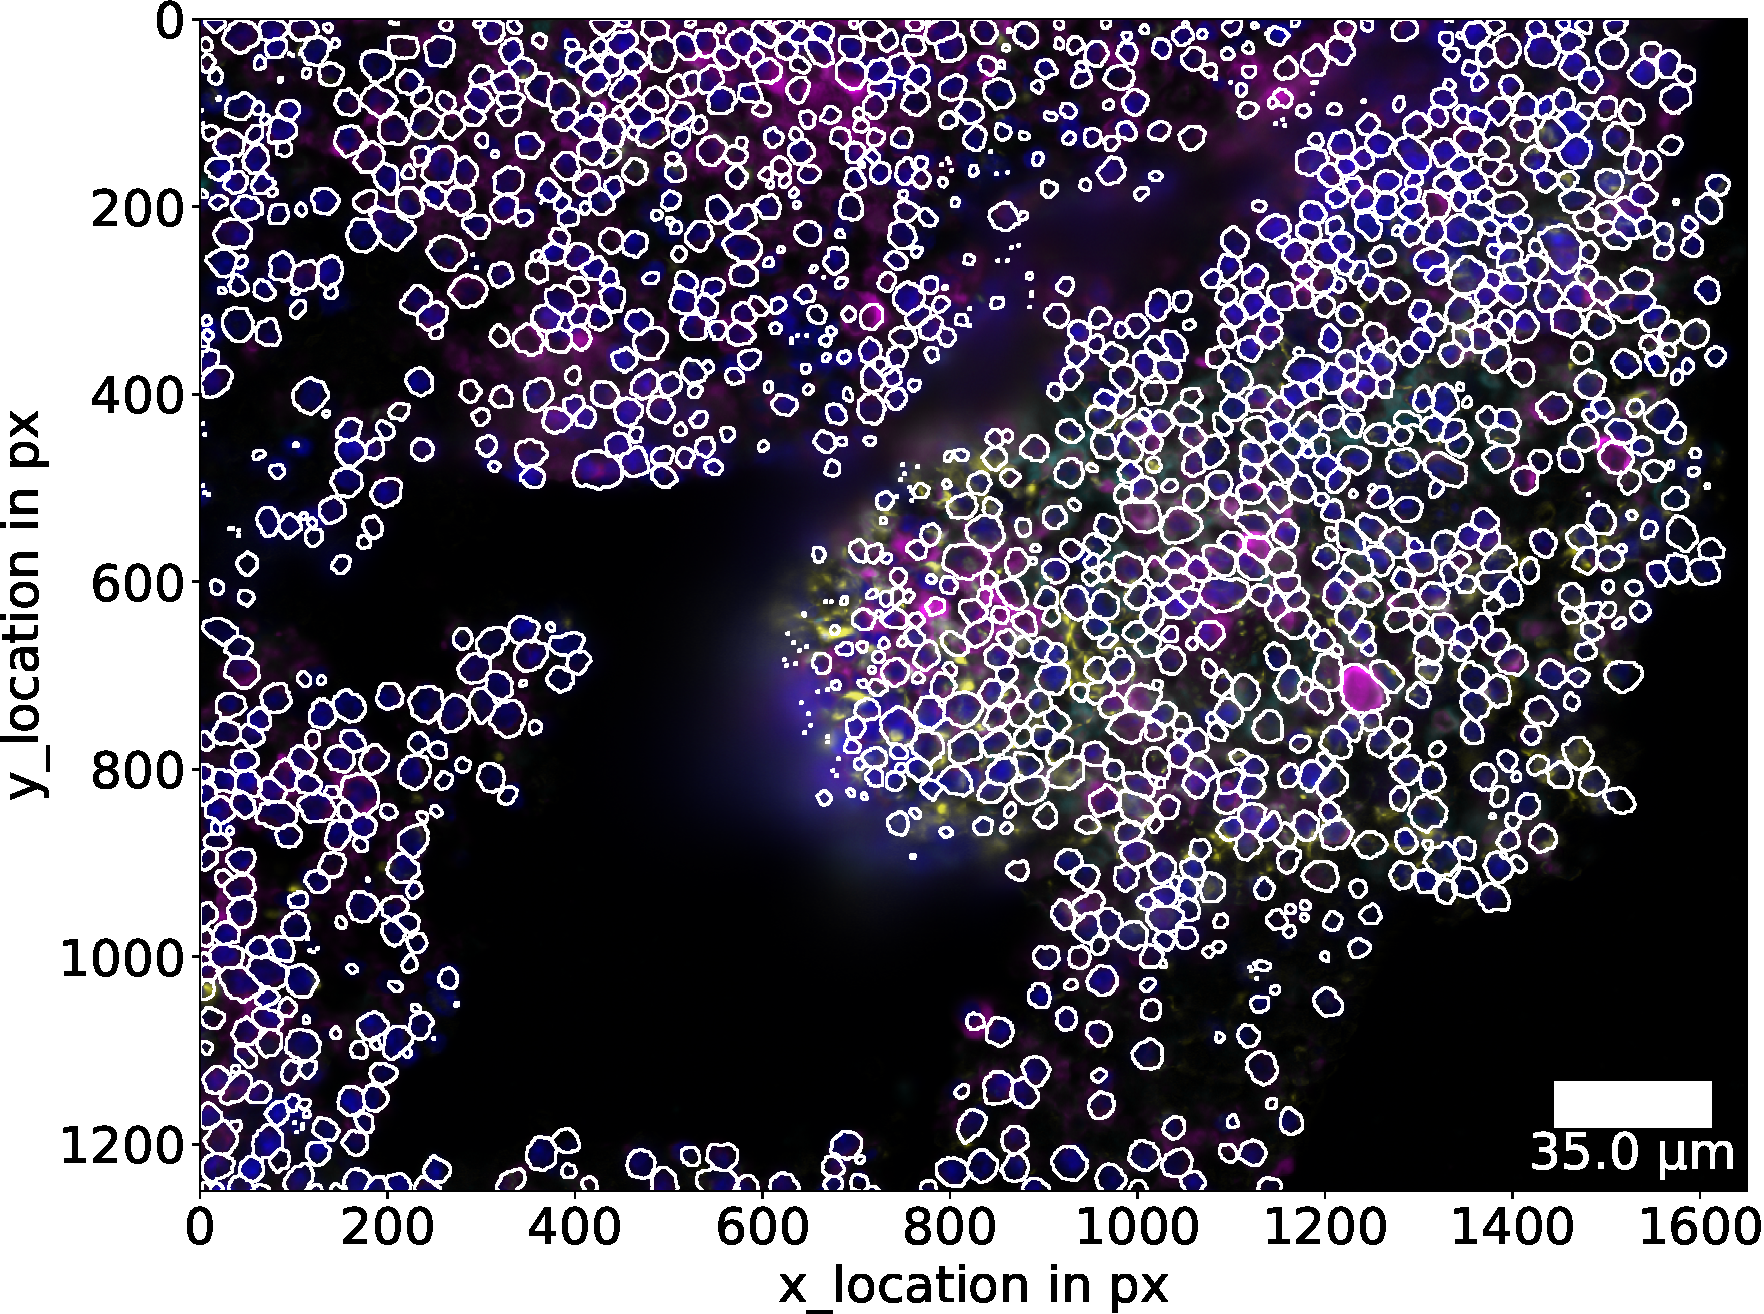
\includegraphics[width=\linewidth]{Images/SI/outlines/outline_proseg_cell-polygon-layers.geojson1.pdf}
        \caption{"Layer 1"-masks  by \textsc{ProSeg}; Input: \inlinepath{transcripts}, located in the section and relative to its origin.}
        \label{fig:Overlay_proseg_1}
    \end{subfigure}%
    \vskip\baselineskip    
    \begin{subfigure}[t]{0.5\textwidth}
        \centering
        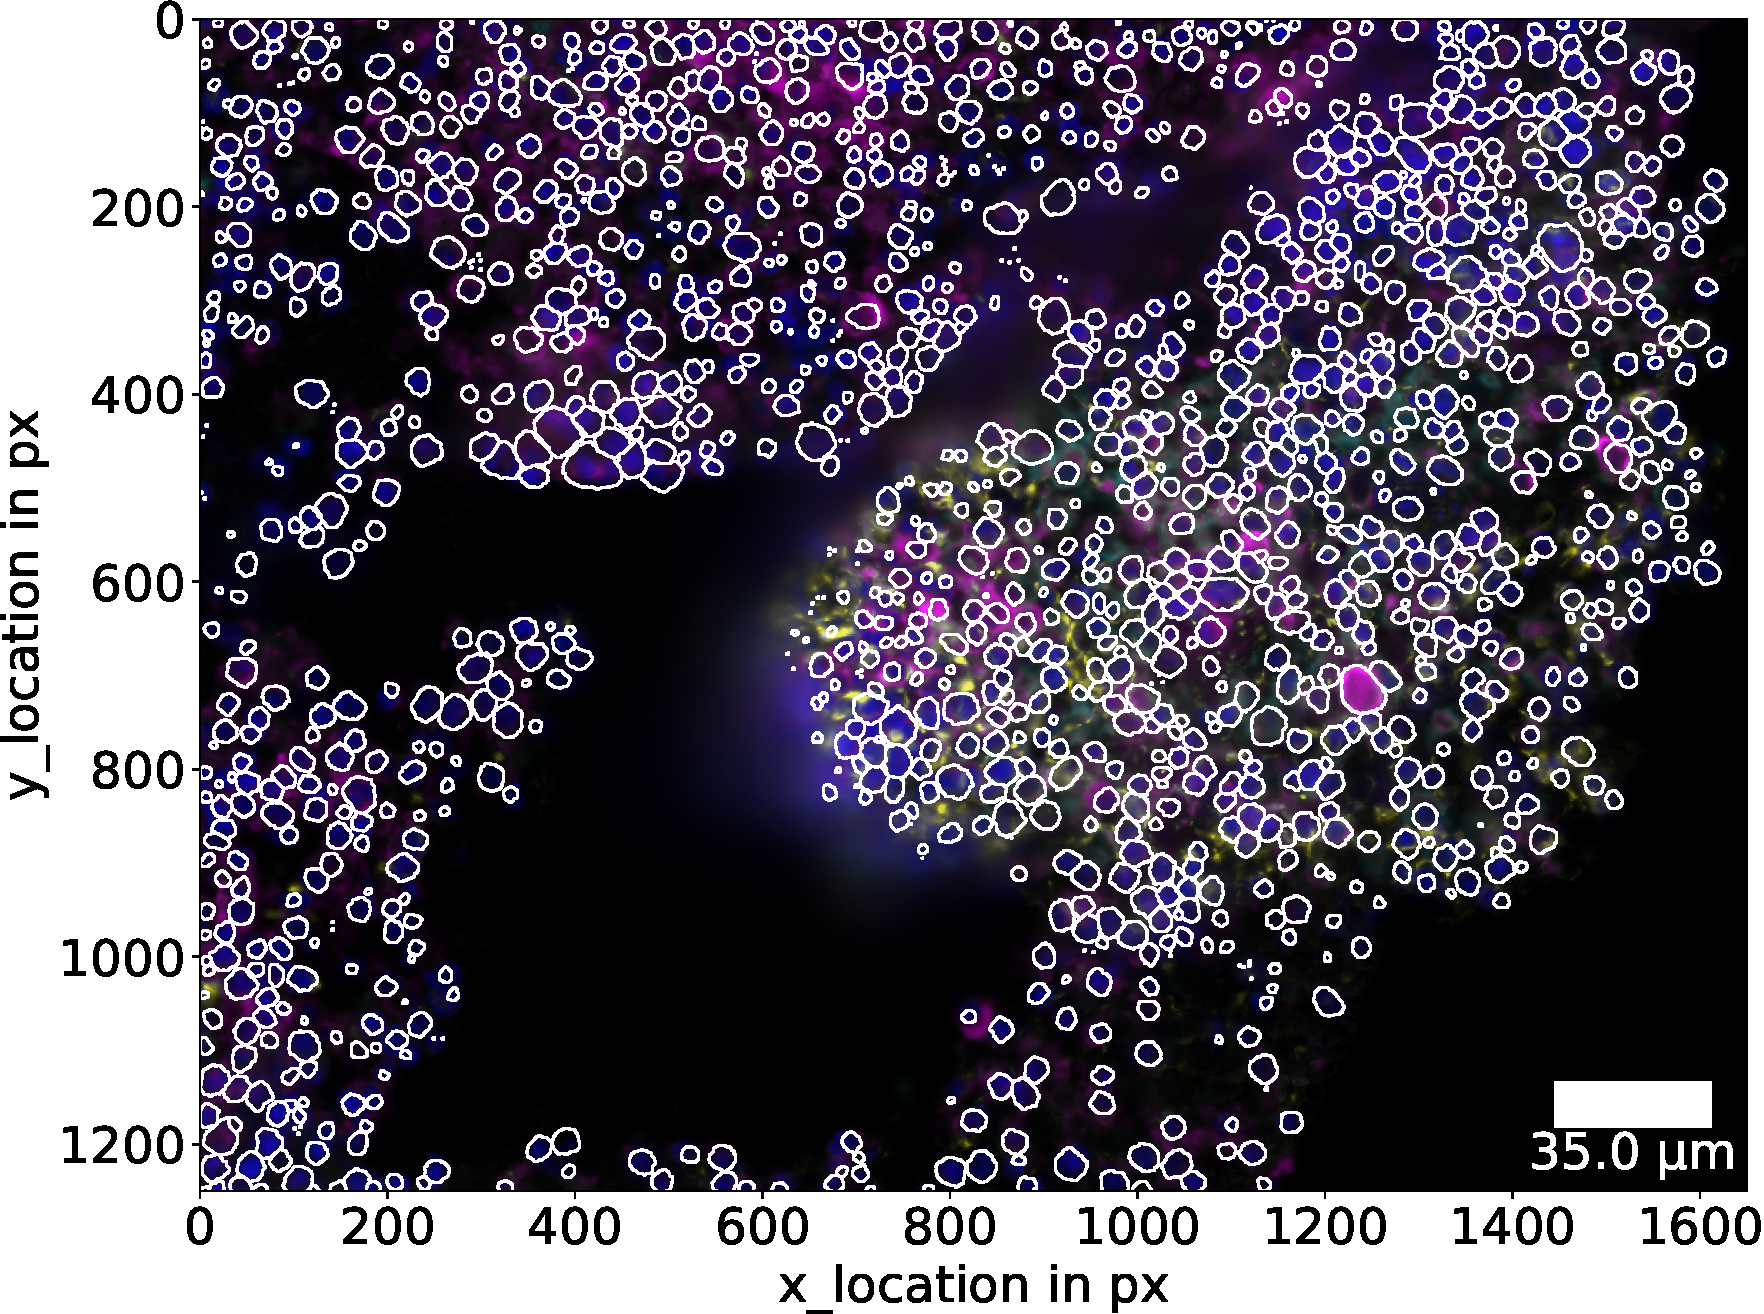
\includegraphics[width=\linewidth]{Images/SI/outlines/outline_proseg_cell-polygon-layers.geojson2.pdf}
        \caption{"Layer 2"-masks  by \textsc{ProSeg}; Input: \inlinepath{transcripts}, located in the section and relative to its origin.}
        \label{fig:Overlay_proseg_2}
    \end{subfigure}%
    ~
    \begin{subfigure}[t]{0.5\textwidth}
        \centering
        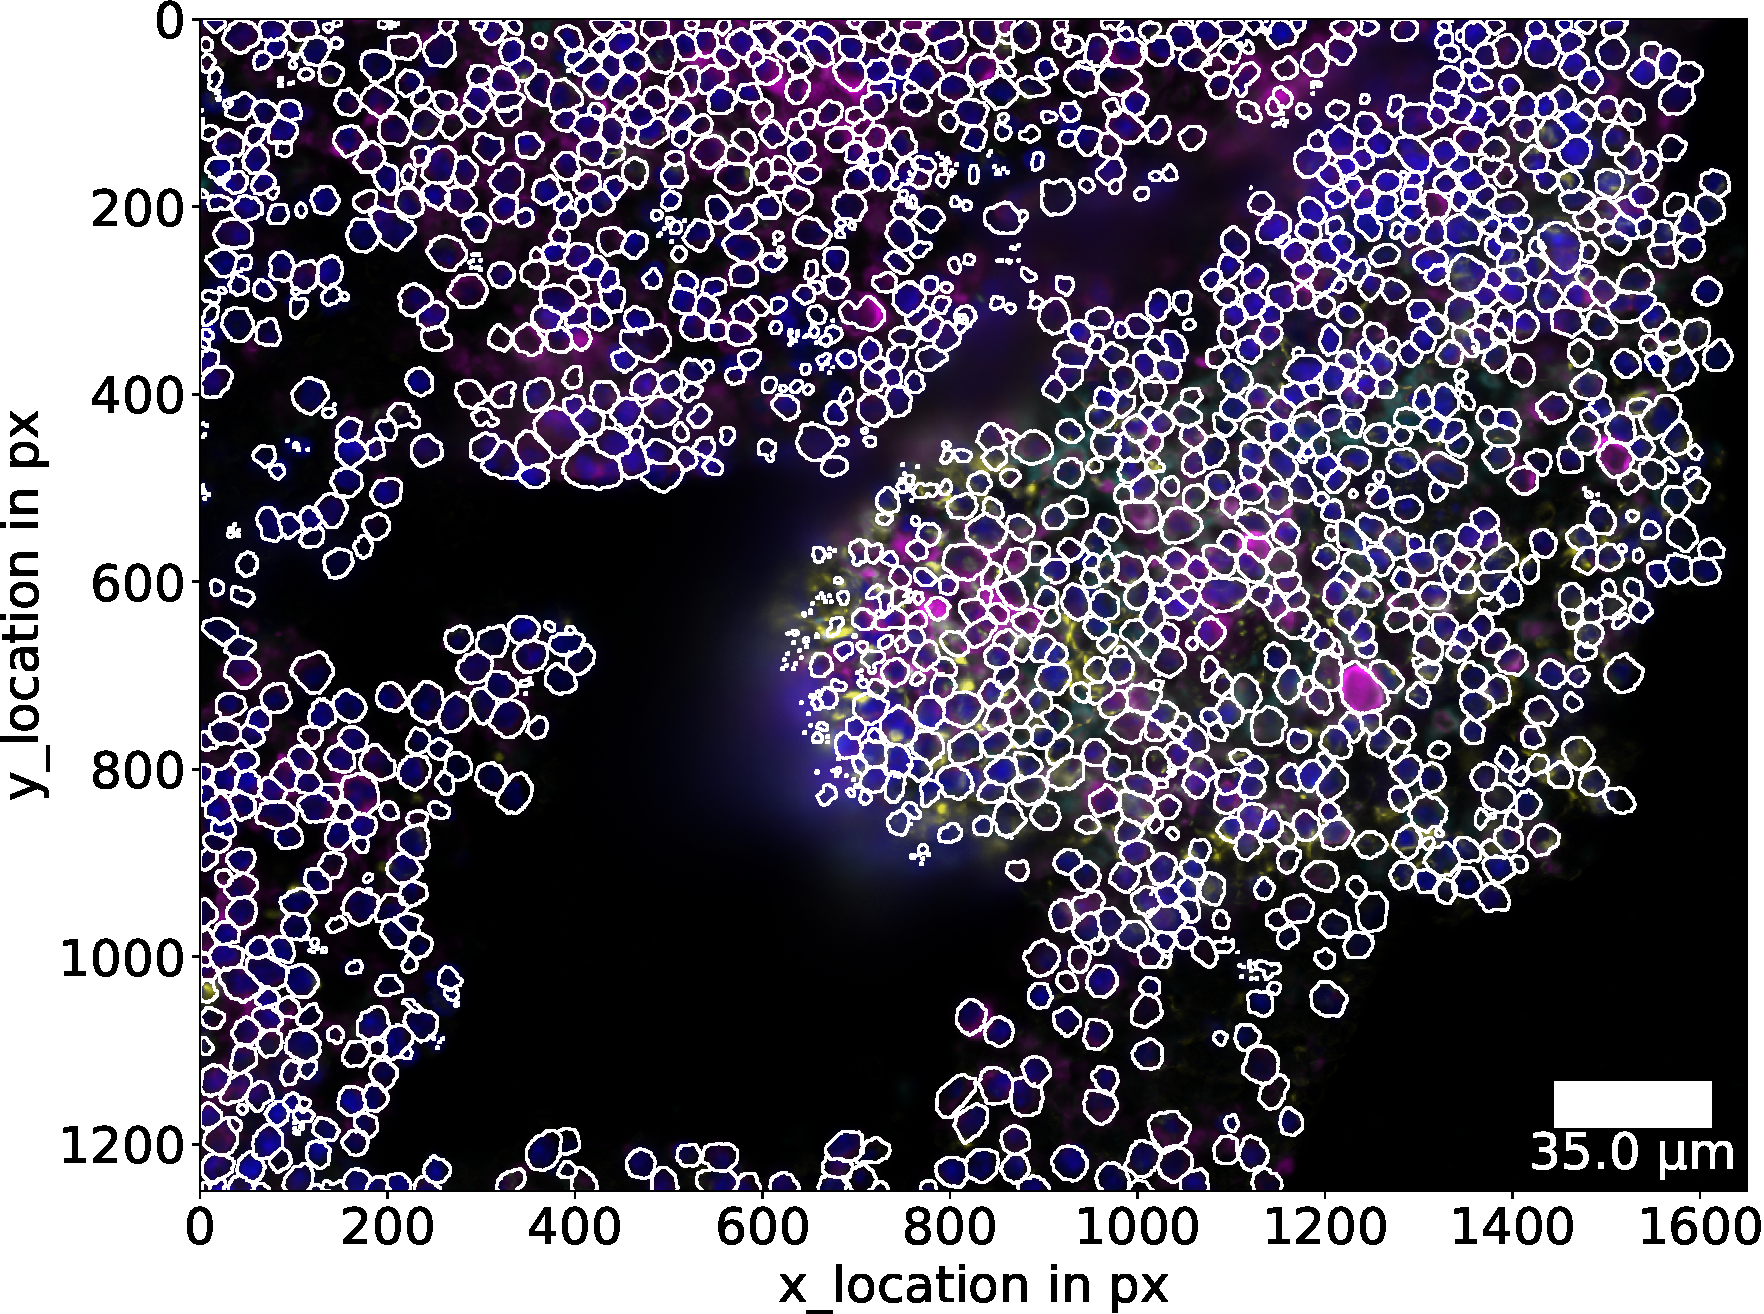
\includegraphics[width=\linewidth]{Images/SI/outlines/outline_proseg_cell-polygons.geojsonall.pdf}
        \caption{Projection of all layers by \textsc{ProSeg}; Input: \inlinepath{transcripts}, located in the section and relative to its origin.}
        \label{fig:Overlay_proseg_a}
    \end{subfigure}
    \caption{Outlines of the predicted masks (white), overlayed on top of the \inlinepath{morphology-focus} image (blue: DAPI; cyan: ATP1A1/CD45/E-Cadherin; magenta: 18s rRNA; yellow: alphaSMA/Vimentin).}
    \label{fig:Outlines_2}
\end{figure*}

\begin{figure*}[t!]
    \begin{subfigure}[t]{0.5\textwidth}
        \centering
        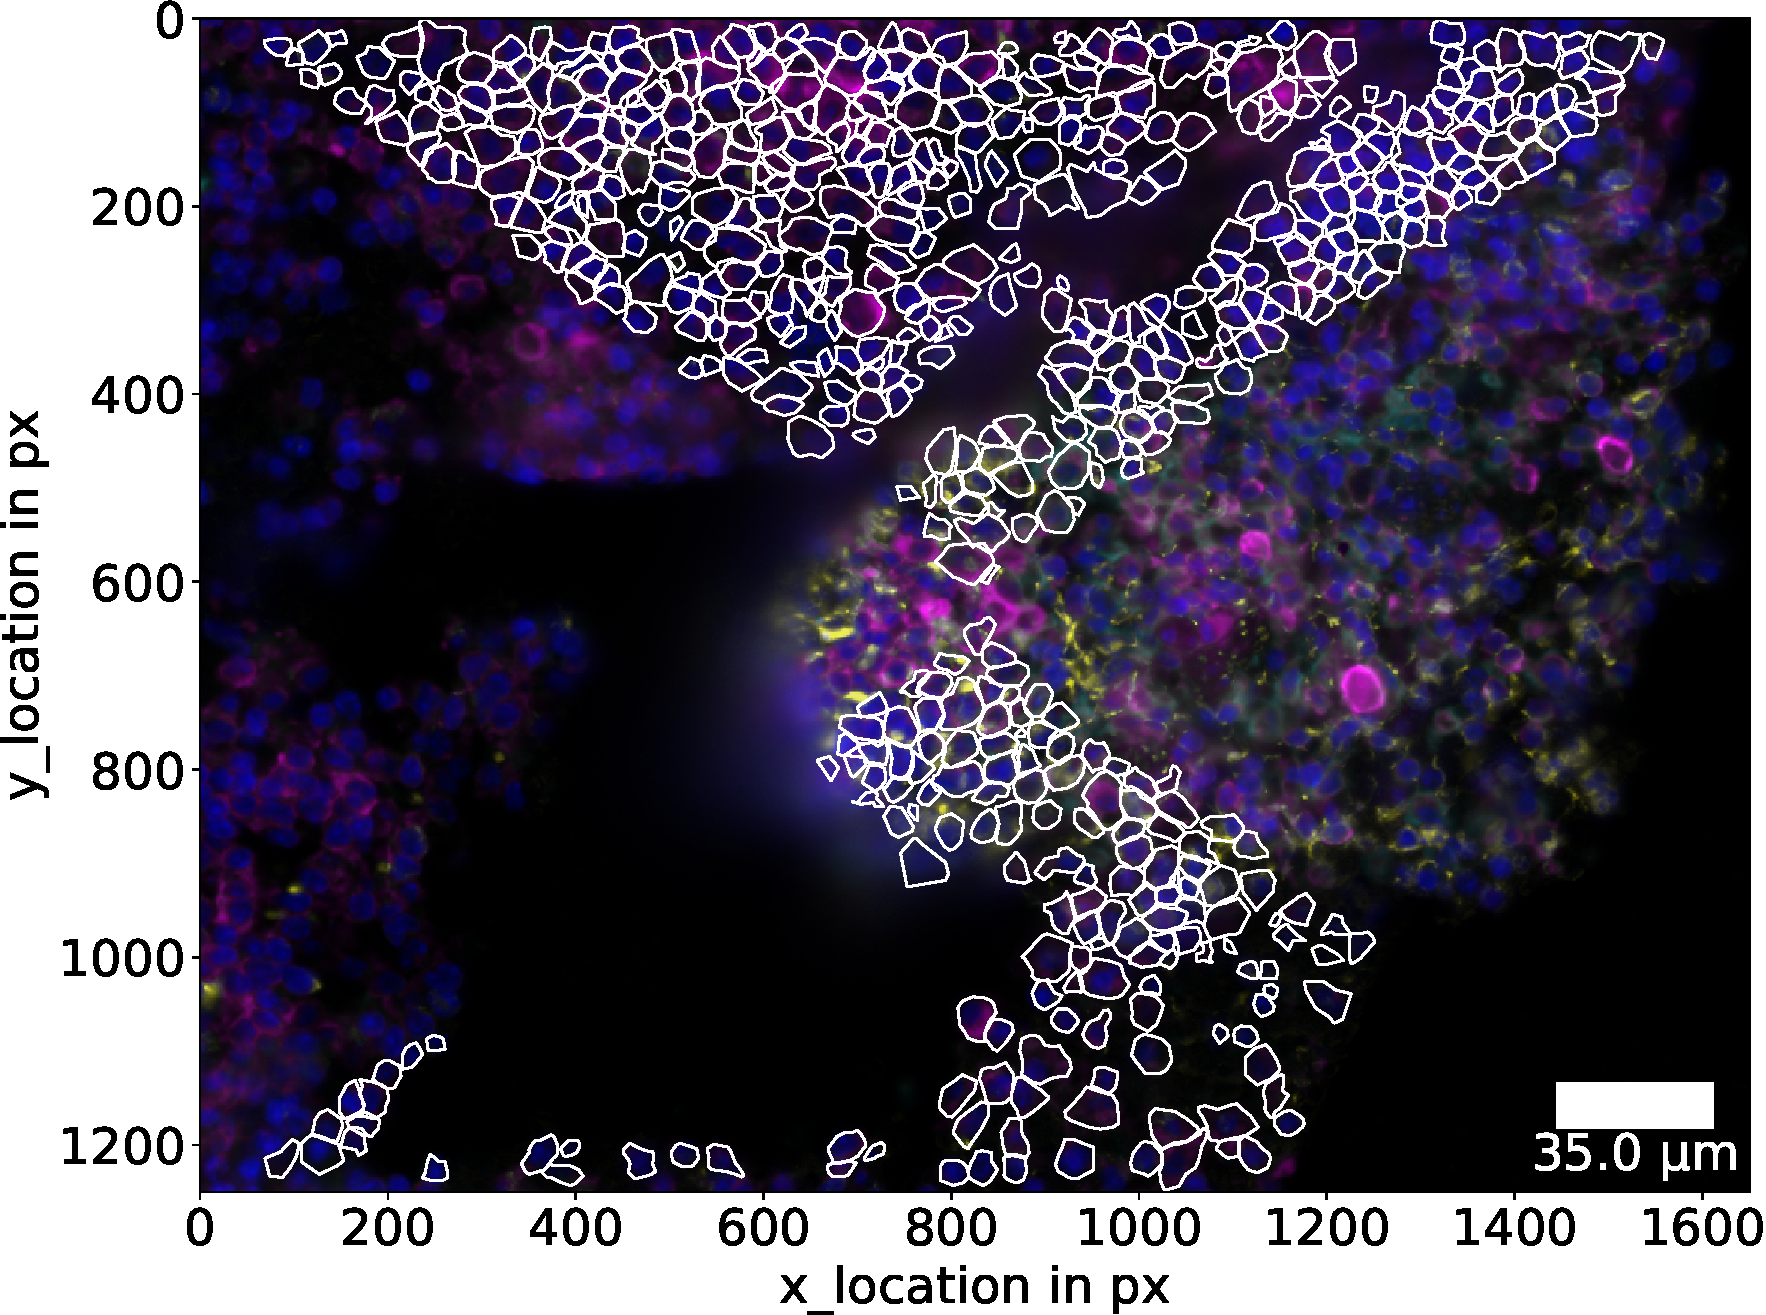
\includegraphics[width=\linewidth]{Images/SI/outlines/outline_segger_cell_polygons.pdf}
        \caption{Cell-masks by \textsc{segger}; Input: \inlinepath{Xenium-output}, unprocessed.}
        \label{fig:Overlay_segger_cel}
    \end{subfigure}%
    ~ 
    \begin{subfigure}[t]{0.5\textwidth}
        \centering
        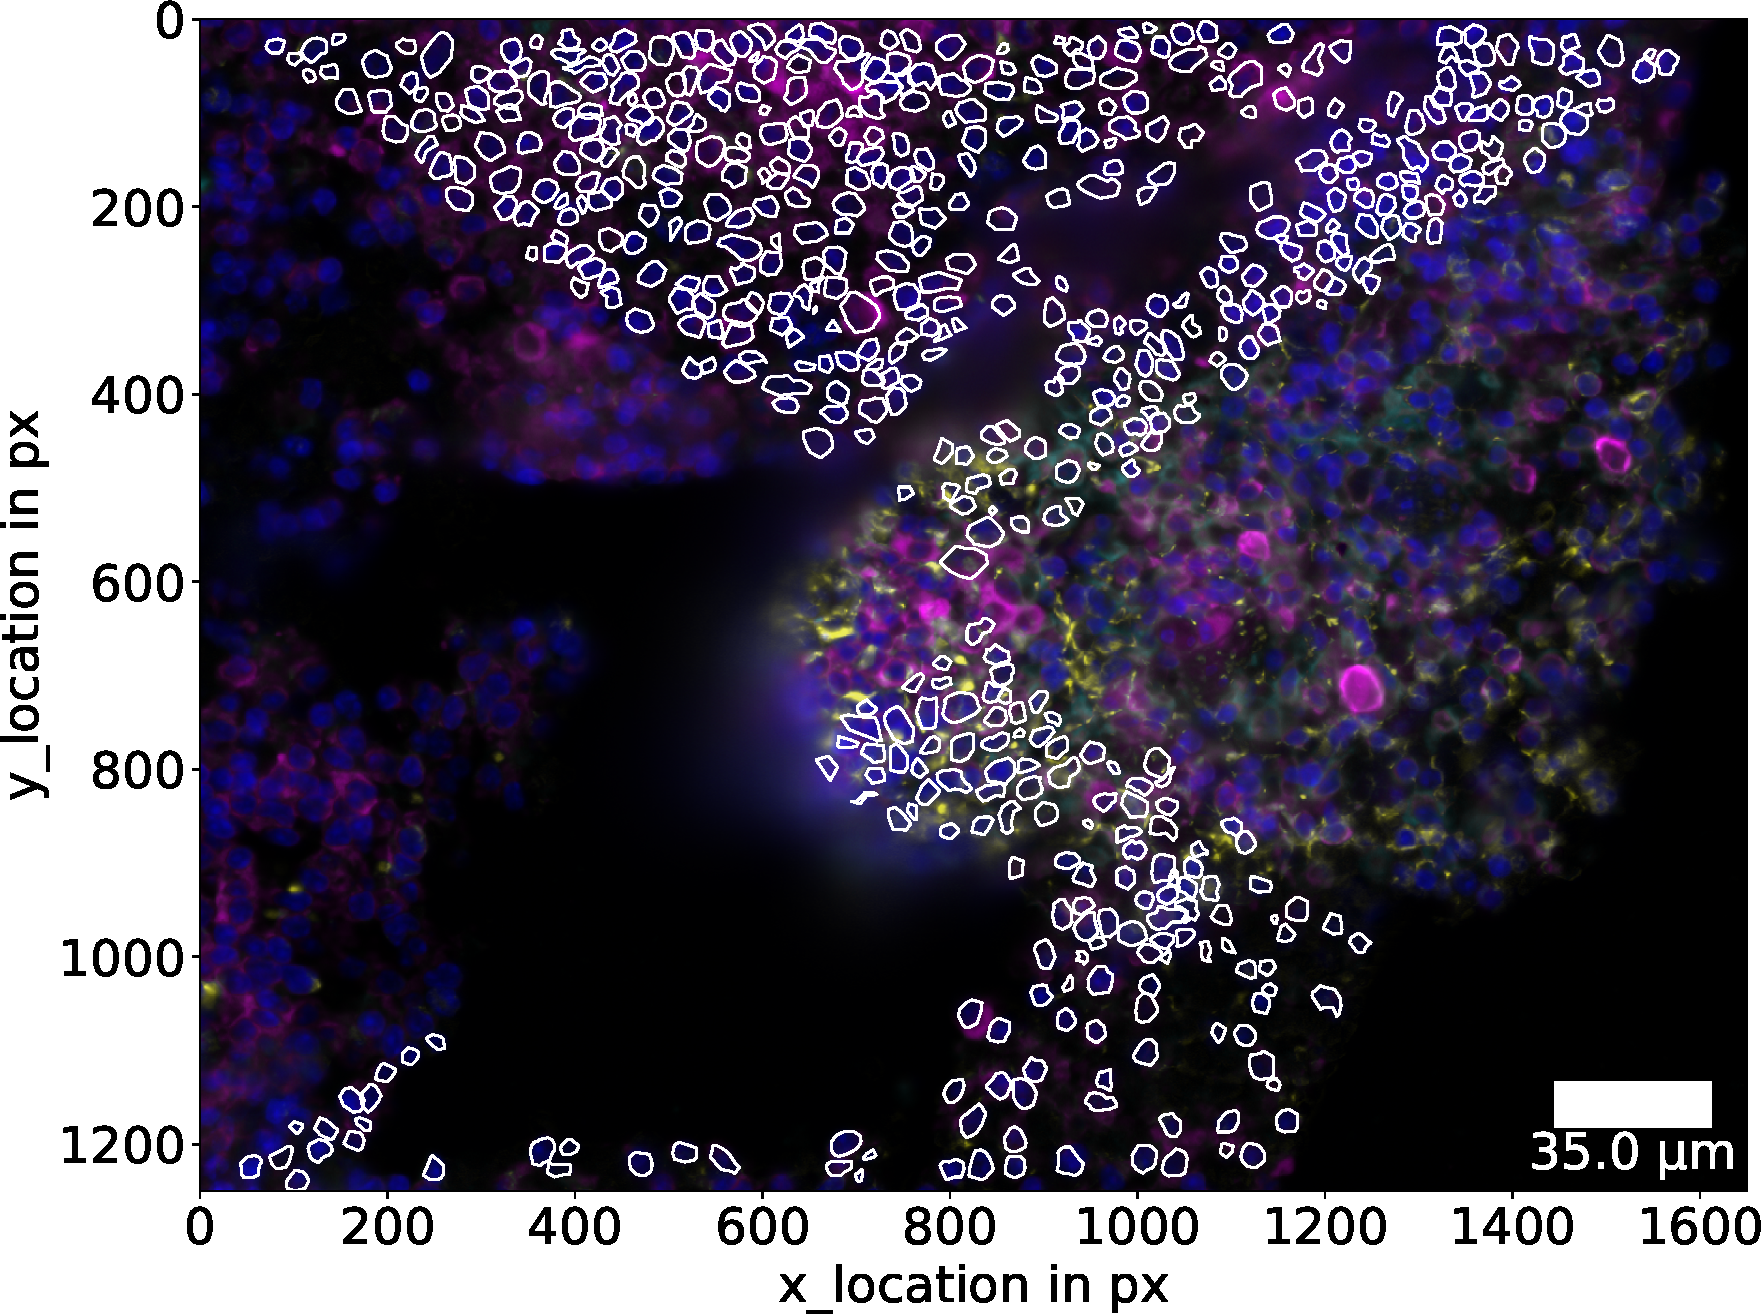
\includegraphics[width=\linewidth]{Images/SI/outlines/outline_segger_nucleus_polygons.pdf}
        \caption{Nucleus-masks by \textsc{segger}; Input: \inlinepath{Xenium-output}, unprocessed.}
        \label{fig:Overlay_segger_nuc}
    \end{subfigure}%
    \vskip\baselineskip
    \begin{subfigure}[t]{0.5\textwidth}
        \centering
        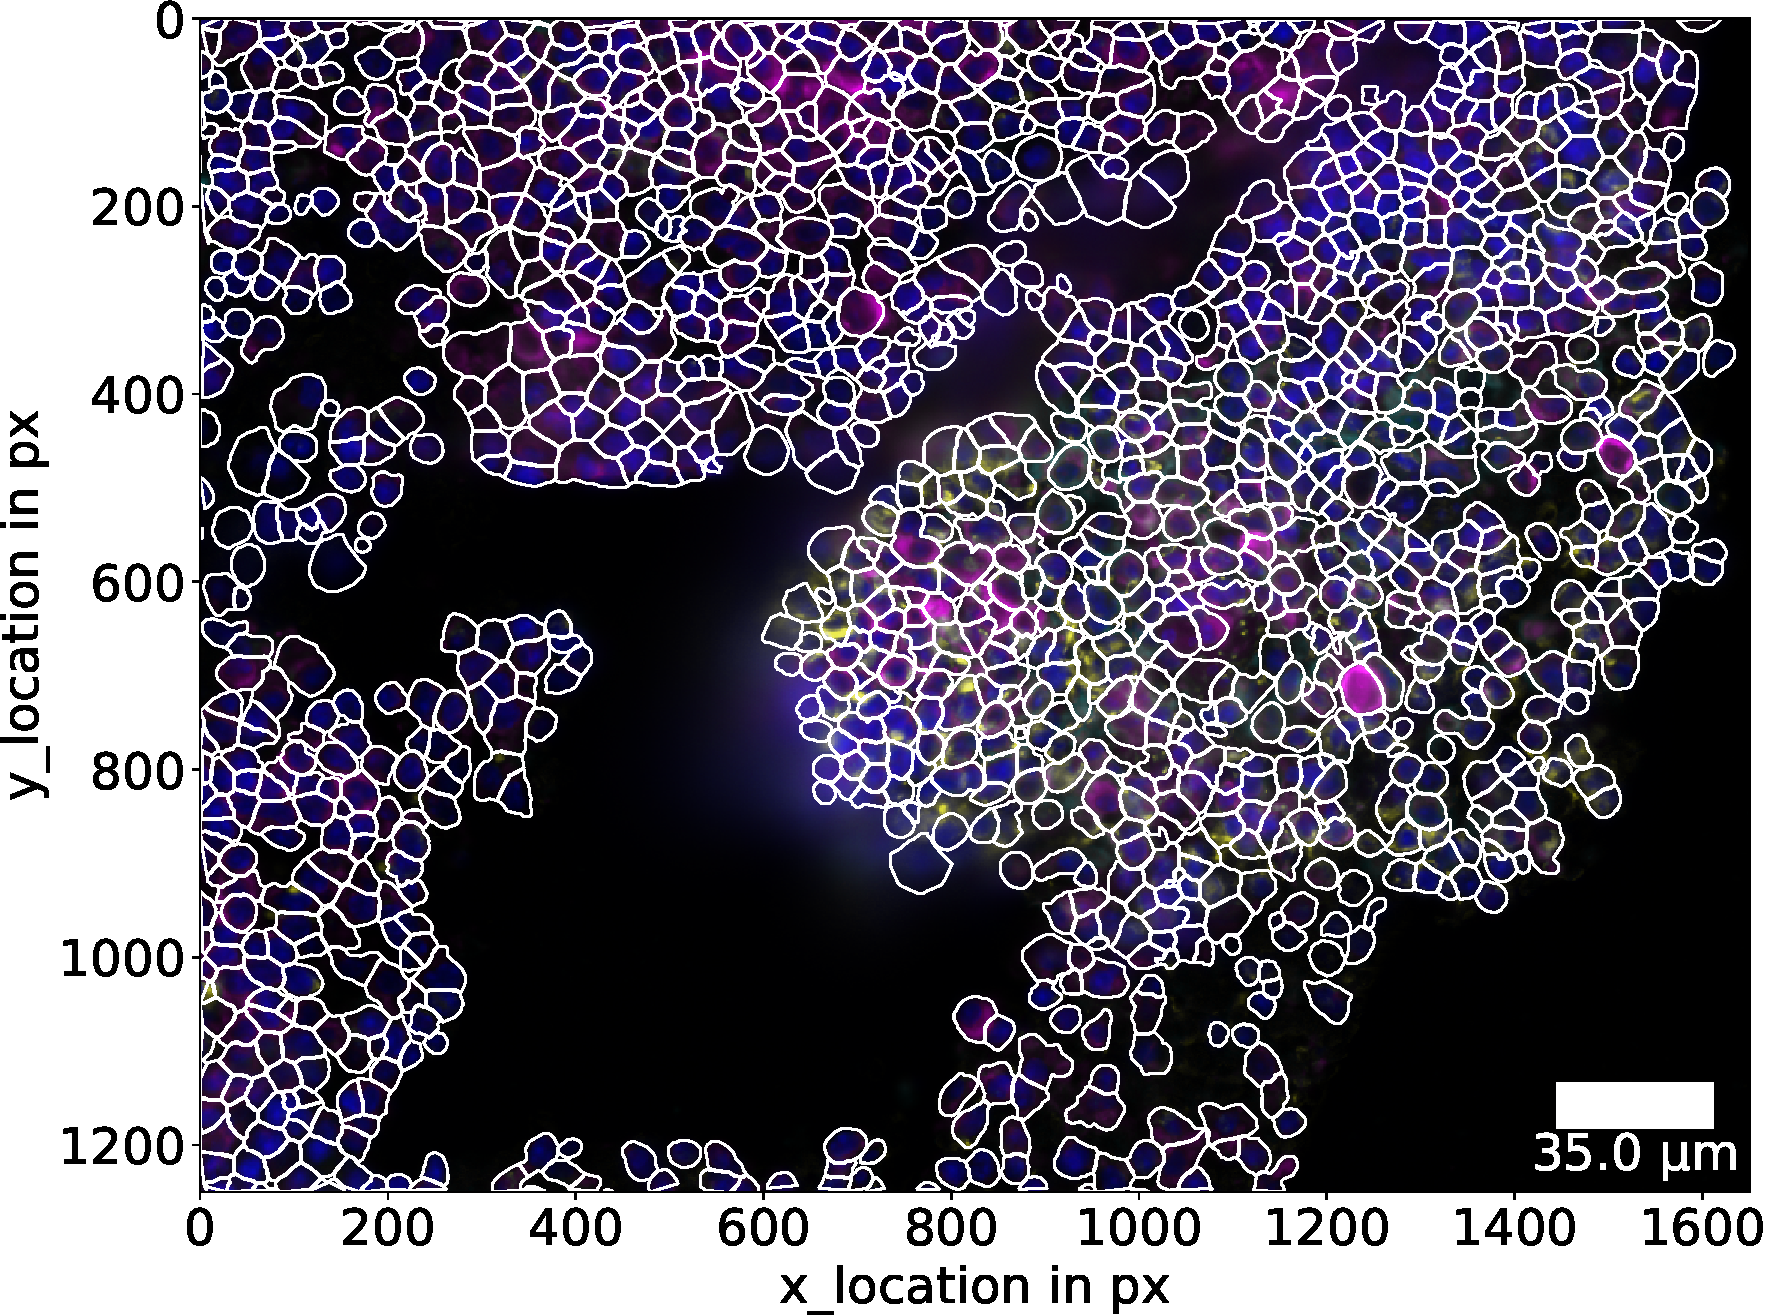
\includegraphics[width=\linewidth]{Images/SI/outlines/outline_xenium_cell_polygons.pdf}
        \caption{Cell-masks by \textsc{XOA}; Input: DAPI, 18s and ATP1A1/CD45/E-Cadherin stainings.}
        \label{fig:Overlay_XOA_cel}
    \end{subfigure}%
    ~
    \begin{subfigure}[t]{0.5\textwidth}
        \centering
        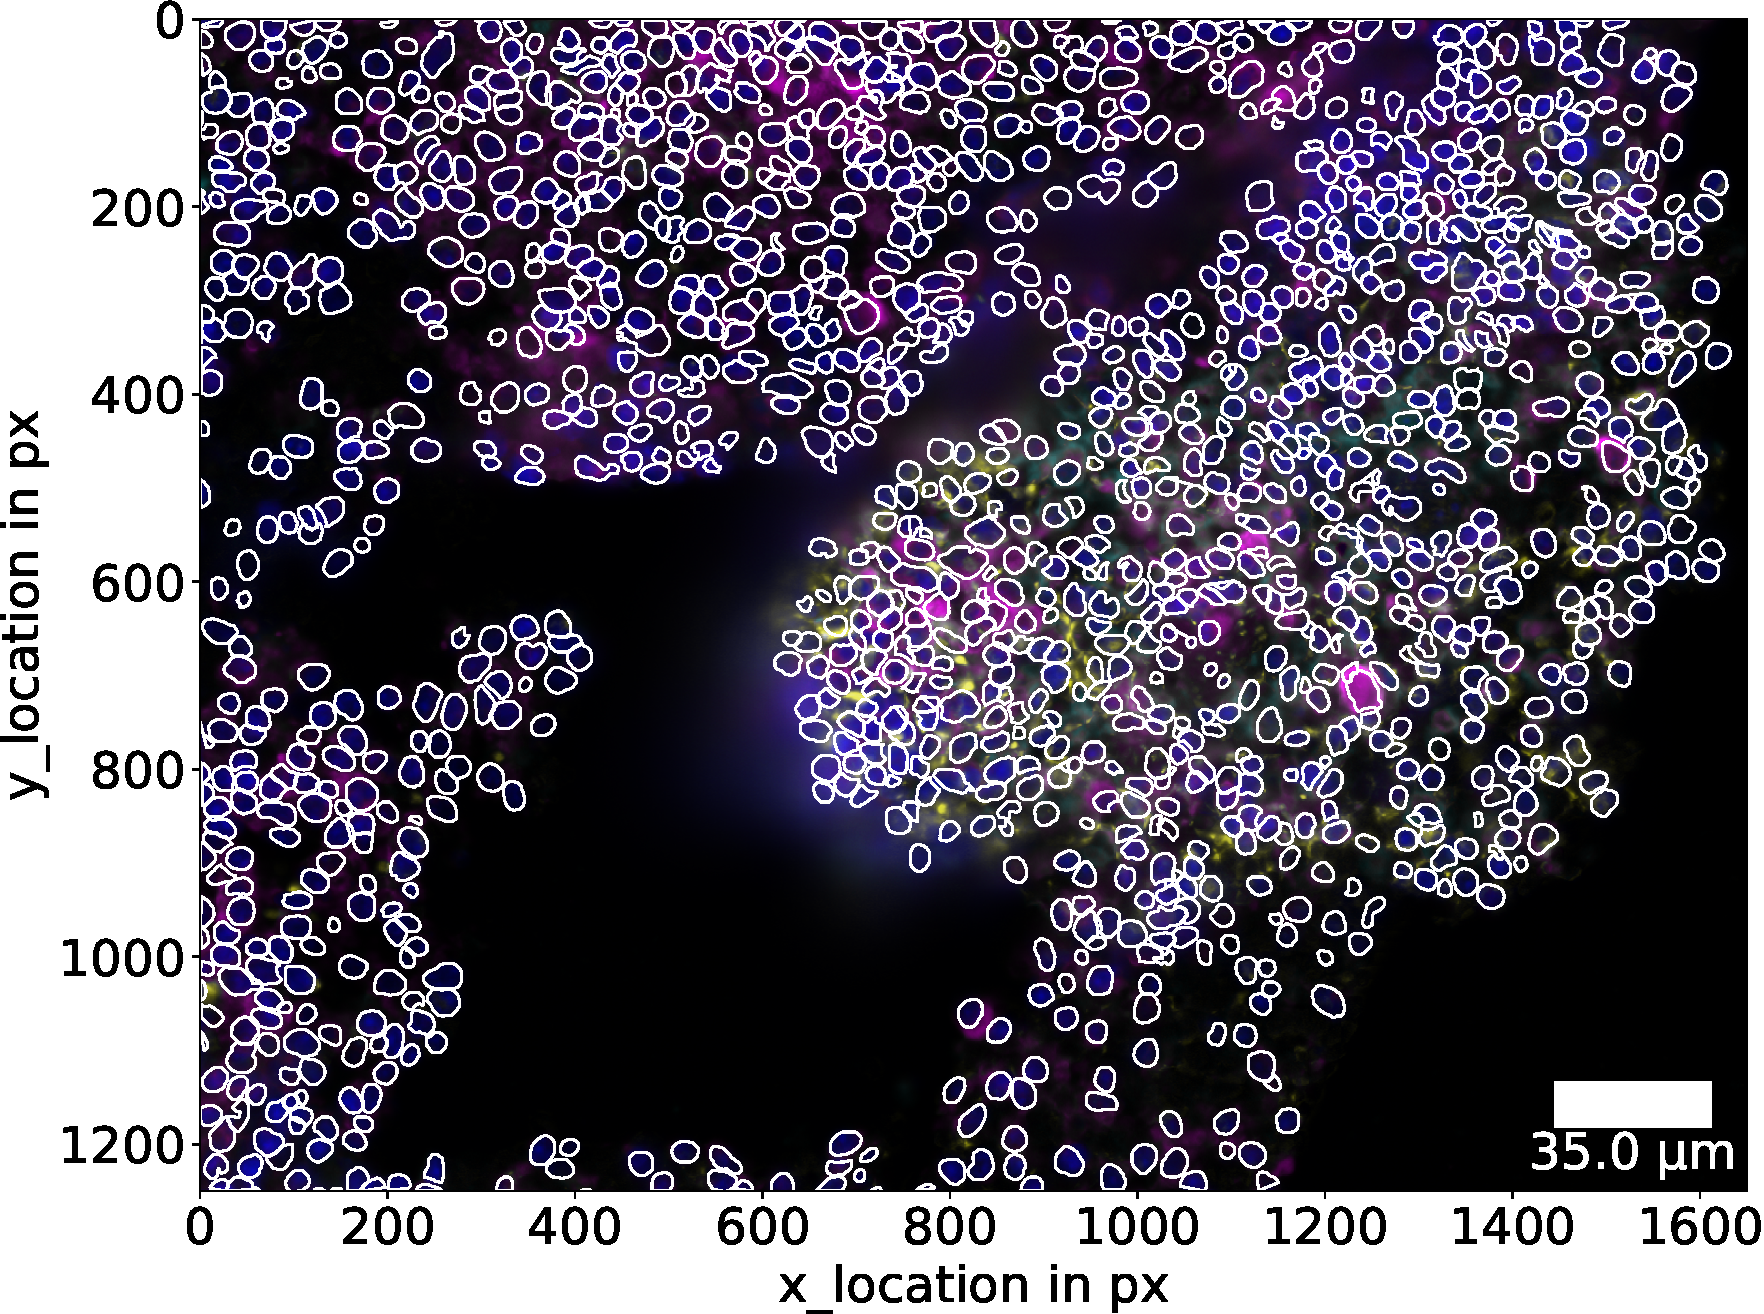
\includegraphics[width=\linewidth]{Images/SI/outlines/outline_xenium_nucleus_polygons.pdf}
        \caption{Nucleus-masks by \textsc{XOA}; Input: DAPI stainings.}
        \label{fig:Overlay_XOA_nuc}
    \end{subfigure}%
    \caption{Outlines of the predicted masks (white), overlayed on top of the \inlinepath{morphology-focus} image (blue: DAPI; cyan: ATP1A1/CD45/E-Cadherin; magenta: 18s rRNA; yellow: alphaSMA/Vimentin).}
    \label{fig:Outlines_3}
\end{figure*}

\subsection*{Panel}
% \newpage
% \begin{table*}[ht]
    \resizebox{\textwidth}{!}{%
    \begin{tabular}{lllrrl}
        \toprule
         & Gene & Ensembl\us ID & Num\us Probesets & Codewords & Annotation \\
        \midrule
        0 & Gpihbp1 & ENSMUSG00000022579 & 8 & 1 & Adipose Tissue - endothelial cell \\
        1 & Mgll & ENSMUSG00000033174 & 8 & 1 & Adipose Tissue - endothelial cell \\
        2 & Iyd & ENSMUSG00000019762 & 9 & 1 & Adipose Tissue - epithelial cell,Trachea - epithelial cell,Large Intestine - epithelial cell of large intestine \\
        3 & Dpt & ENSMUSG00000026574 & 8 & 1 & Adipose Tissue - mesenchymal stem cell of adipose tissue \\
        4 & Lum & ENSMUSG00000036446 & 8 & 1 & Adipose Tissue - mesenchymal stem cell of adipose tissue \\
        5 & Retn & ENSMUSG00000012705 & 8 & 1 & Adipose Tissue - myeloid cell \\
        6 & Retnla & ENSMUSG00000061100 & 8 & 1 & Adipose Tissue - myeloid cell,Lung - lung macrophage \\
        7 & Car3 & ENSMUSG00000027559 & 8 & 1 & Bladder Lumen - bladder cell,Adipose Tissue - mesenchymal stem cell of adipose tissue \\
        8 & Nbl1 & ENSMUSG00000041120 & 8 & 1 & Bladder Lumen - bladder cell,Adipose Tissue - mesenchymal stem cell of adipose tissue \\
        9 & Asz1 & ENSMUSG00000010796 & 8 & 1 & Bladder Lumen - bladder cell,Lung - adventitial cell \\
        10 & Cldn4 & ENSMUSG00000047501 & 7 & 1 & Bladder Lumen - bladder urothelial cell \\
        11 & Areg & ENSMUSG00000029378 & 9 & 1 & Bladder Lumen - bladder urothelial cell,Lung - lung macrophage \\
        12 & Aqp3 & ENSMUSG00000028435 & 8 & 1 & Bladder Lumen - bladder urothelial cell,Skin of Body - stem cell of epidermis \\
        13 & Ivl & ENSMUSG00000049128 & 9 & 1 & Bladder Lumen - bladder urothelial cell,Skin of Body - stem cell of epidermis \\
        14 & Cyp11a1 & ENSMUSG00000032323 & 8 & 1 & Bone Marrow - basophil,Lung - basophil \\
        15 & Ccl9 & ENSMUSG00000019122 & 8 & 1 & Bone Marrow - basophil,Lung - basophil,Large Intestine - intestinal macrophage \\
        16 & Hmbs & ENSMUSG00000032126 & 8 & 1 & Bone Marrow - erythroblast,Adipose Tissue - erythroblast,Spleen - erythroblast \\
        17 & Rhd & ENSMUSG00000028825 & 8 & 1 & Bone Marrow - erythroblast,Adipose Tissue - erythroblast,Spleen - erythroblast \\
        18 & Hemgn & ENSMUSG00000028332 & 8 & 1 & Bone Marrow - erythroblast,Adipose Tissue - erythroblast,Spleen - erythroblast,Large Intestine - hematopoietic stem cell large \\
        19 & Ctse & ENSMUSG00000004552 & 8 & 1 & Bone Marrow - erythroblast,Adipose Tissue - erythroblast,Spleen - erythroblast,Large Intestine - large intestine goblet cell \\
        20 & Ifitm6 & ENSMUSG00000059108 & 8 & 1 & Bone Marrow - granulocyte,Spleen - granulocyte,Trachea - granulocyte \\
        21 & Pglyrp1 & ENSMUSG00000030413 & 5 & 1 & Bone Marrow - granulocyte,Spleen - granulocyte,Trachea - granulocyte \\
        22 & Ube2c & ENSMUSG00000001403 & 8 & 1 & Bone Marrow - granulocytopoietic cell,Large Intestine - hematopoietic stem cell large \\
        23 & Rac2 & ENSMUSG00000033220 & 8 & 1 & Bone Marrow - hematopoietic precursor cell,Large Intestine - hematopoietic stem cell large \\
        24 & Ctla2a & ENSMUSG00000044258 & 8 & 1 & Bone Marrow - hematopoietic precursor cell,Lung - T cell,Skin of Body - T cell,Limb Muscle - T cell \\
        25 & Slc25a37 & ENSMUSG00000034248 & 8 & 1 & Bone Marrow - immature B cell \\
        26 & Slc4a1 & ENSMUSG00000006574 & 8 & 1 & Bone Marrow - immature B cell \\
        27 & Ms4a7 & ENSMUSG00000024672 & 8 & 1 & Bone Marrow - macrophage,Mammary Gland - macrophage,Kidney - macrophage,Limb Muscle - macrophage,Spleen - macrophage,Trachea - macrophage \\
        28 & Fcnb & ENSMUSG00000026835 & 8 & 1 & Bone Marrow - megakaryocyte-erythroid progenitor cell,Spleen - megakaryocyte-erythroid progenitor cell \\
        29 & Cpa3 & ENSMUSG00000001865 & 8 & 1 & Bone Marrow - naive B cell \\
        30 & Klra8 & ENSMUSG00000089727 & 8 & 1 & Bone Marrow - natural killer cell,Kidney - natural killer cell,Liver - natural killer cell,Lung - natural killer cell,Spleen - natural killer cell \\
        31 & Prg2 & ENSMUSG00000027073 & 8 & 1 & Bone Marrow - plasma cell,Kidney - plasma cell,Lung - plasma cell,Spleen - plasma cell \\
        32 & Mmp8 & ENSMUSG00000005800 & 9 & 1 & Bone Marrow - proerythroblast,Spleen - proerythroblast \\
        33 & Hp & ENSMUSG00000031722 & 6 & 1 & Bone Marrow - promonocyte,Lung - endothelial cell of lymphatic vessel,Liver - hepatocyte \\
        34 & Gfap & ENSMUSG00000020932 & 8 & 1 & Brain - astrocyte \\
        35 & Gad1 & ENSMUSG00000070880 & 9 & 1 & Brain - GABAergic neuron \\
        36 & Pvalb & ENSMUSG00000005716 & 4 & 1 & Brain - GABAergic neuron \\
        37 & Pou3f3 & ENSMUSG00000045515 & 8 & 1 & Brain - glutamatergic neuron \\
        38 & Slc17a7 & ENSMUSG00000070570 & 8 & 1 & Brain - glutamatergic neuron \\
        39 & Cux2 & ENSMUSG00000042589 & 8 & 1 & Brain - granule cell layer neuron \\
        40 & Sox2 & ENSMUSG00000074637 & 9 & 1 & Brain - neural stem cell \\
        41 & Tubb3 & ENSMUSG00000062380 & 8 & 1 & Brain - sensory ganglia \\
        42 & Prox1 & ENSMUSG00000010175 & 9 & 1 & Eye - lens of eye \\
        43 & Vsx2 & ENSMUSG00000021239 & 9 & 1 & Eye - lens of eye \\
        44 & Rho & ENSMUSG00000030324 & 9 & 1 & Eye - rod cells of the retina \\
        45 & Pln & ENSMUSG00000038583 & 8 & 1 & Heart - cadiac muscle cell \\
        46 & Hrc & ENSMUSG00000038239 & 8 & 1 & Heart - cardiac muscle cell \\
        47 & Mylk3 & ENSMUSG00000031698 & 8 & 1 & Heart - cardiac muscle cell \\
        48 & Myoz2 & ENSMUSG00000028116 & 8 & 1 & Heart - cardiac muscle cell \\
        49 & Trdn & ENSMUSG00000019787 & 8 & 1 & Heart - cardiac muscle cell \\
        50 & Ttn & ENSMUSG00000051747 & 9 & 1 & Heart - cardiac muscle cell \\
        51 & Mapk10 & ENSMUSG00000046709 & 9 & 1 & Heart - cardiac muscle cell,Brain - glutamatergic neuron,Brain - GABAergic neuron \\
        52 & Tnnc1 & ENSMUSG00000091898 & 5 & 1 & Heart - cardiac muscle cell,Limb Muscle - cell of skeletal muscle \\
        53 & Cox8b & ENSMUSG00000025488 & 2 & 1 & Heart - cardiac muscle cell,Limb Muscle - endothelial cell \\
        54 & Chl1 & ENSMUSG00000030077 & 9 & 1 & Heart - cardiac neuron \\
        55 & Fxyd1 & ENSMUSG00000036570 & 1 & 1 & Heart - cardiac neuron \\
        56 & Kcna1 & ENSMUSG00000047976 & 8 & 1 & Heart - cardiac neuron \\
        57 & Plp1 & ENSMUSG00000031425 & 2 & 1 & Heart - cardiac neuron \\
        58 & Ppbp & ENSMUSG00000029372 & 8 & 1 & Heart - cardiac neuron \\
        59 & Comp & ENSMUSG00000031849 & 8 & 1 & Heart - endocardial cell \\
        60 & Cfh & ENSMUSG00000026365 & 8 & 1 & Heart - endocardial cell,Adipose Tissue - mesenchymal stem cell of adipose tissue \\
        61 & Eng & ENSMUSG00000026814 & 8 & 1 & Heart - endocardial cell,Limb Muscle - mesenchymal stem cell \\
        62 & Aqp7 & ENSMUSG00000028427 & 8 & 1 & Heart - endothelial cell of coronary artery \\
        63 & Rbp7 & ENSMUSG00000028996 & 4 & 1 & Heart - endothelial cell of coronary artery \\
        64 & Tcf15 & ENSMUSG00000068079 & 2 & 1 & Heart - endothelial cell of coronary artery \\
        65 & Timp4 & ENSMUSG00000030317 & 8 & 1 & Heart - endothelial cell of coronary artery \\
        66 & Car2 & ENSMUSG00000027562 & 4 & 1 & Heart - erythrocyte \\
        67 & Fech & ENSMUSG00000024588 & 8 & 1 & Heart - erythrocyte \\
        68 & Isca1 & ENSMUSG00000044792 & 8 & 1 & Heart - erythrocyte \\
        69 & Isg20 & ENSMUSG00000039236 & 4 & 1 & Heart - erythrocyte \\
        70 & Pi16 & ENSMUSG00000024011 & 8 & 1 & Heart - fibroblast of cardiac tissue \\
        71 & Serpina3n & ENSMUSG00000021091 & 8 & 1 & Heart - fibroblast of cardiac tissue \\
        72 & Ccdc80 & ENSMUSG00000022665 & 8 & 1 & Heart - fibroblast of cardiac tissue,Trachea - fibroblast \\
        73 & Ccl12 & ENSMUSG00000035352 & 5 & 1 & Heart - leukocyte,Pancreas - leukocyte,Bladder Lumen - leukocyte,Kidney - leukocyte \\
        74 & F13a1 & ENSMUSG00000039109 & 8 & 1 & Heart - leukocyte,Pancreas - leukocyte,Bladder Lumen - leukocyte,Kidney - leukocyte \\
        75 & Asprv1 & ENSMUSG00000033508 & 8 & 1 & Heart - mast cell \\
        76 & C5ar1 & ENSMUSG00000049130 & 8 & 1 & Heart - mast cell \\
        77 & Mrgpra2a & ENSMUSG00000093973 & 8 & 1 & Heart - mast cell \\
        78 & Cstdc4 & ENSMUSG00000079597 & 6 & 1 & Heart - mast cell,Skin of Body - basal cell of epidermis \\
        79 & Stfa2l1 & ENSMUSG00000059657 & 4 & 1 & Heart - mast cell,Skin of Body - basal cell of epidermis \\
        80 & Myh11 & ENSMUSG00000018830 & 8 & 1 & Heart - smooth muscle cell,Limb Muscle - smooth muscle cell \\
        81 & Aadat & ENSMUSG00000057228 & 9 & 1 & Kidney - brush cell \\
        82 & Cubn & ENSMUSG00000026726 & 8 & 1 & Kidney - brush cell \\
        83 & Hsd3b4 & ENSMUSG00000095143 & 8 & 1 & Kidney - brush cell \\
        84 & Mettl7a2 & ENSMUSG00000056487 & 8 & 1 & Kidney - brush cell \\
        85 & Slc27a2 & ENSMUSG00000027359 & 8 & 1 & Kidney - brush cell \\
        86 & 0610005C13Rik & ENSMUSG00000109644 & 6 & 1 & Kidney - epithelial cell of proximal tubule \\
        87 & Cndp2 & ENSMUSG00000024644 & 8 & 1 & Kidney - epithelial cell of proximal tubule \\
        88 & Guca2b & ENSMUSG00000032978 & 5 & 1 & Kidney - epithelial cell of proximal tubule \\
        89 & Ttc36 & ENSMUSG00000039438 & 2 & 1 & Kidney - epithelial cell of proximal tubule \\
        90 & Slc22a6 & ENSMUSG00000024650 & 9 & 1 & Kidney - epithelial cell of proximal tubule,Brain - astrocyte \\
        91 & AU021092 & ENSMUSG00000051669 & 8 & 1 & Kidney - fenestrated cell \\
        92 & Tie1 & ENSMUSG00000033191 & 8 & 1 & Kidney - fenestrated cell \\
        93 & Plvap & ENSMUSG00000034845 & 9 & 1 & Kidney - fenestrated cell,Lung - type II pneumocyte \\
        94 & Col8a1 & ENSMUSG00000068196 & 8 & 1 & Kidney - fibroblast,Trachea - fibroblast \\
        95 & Otor & ENSMUSG00000027416 & 8 & 1 & Kidney - fibroblast,Trachea - fibroblast \\
        96 & Wif1 & ENSMUSG00000020218 & 8 & 1 & Kidney - fibroblast,Trachea - fibroblast \\
        97 & Kdr & ENSMUSG00000062960 & 9 & 1 & Kidney - kidney capillary endothelial cell \\
        98 & Clec4a3 & ENSMUSG00000043832 & 9 & 1 & Kidney - kidney cell \\
        99 & Ncf4 & ENSMUSG00000071715 & 8 & 1 & Kidney - kidney cell \\
        100 & Abca13 & ENSMUSG00000004668 & 8 & 1 & Kidney - kidney collecting duct epithelial cell \\
        101 & Kcnj16 & ENSMUSG00000051497 & 8 & 1 & Kidney - kidney collecting duct epithelial cell \\
        102 & Kl & ENSMUSG00000058488 & 9 & 1 & Kidney - kidney collecting duct epithelial cell \\
        103 & Pgam2 & ENSMUSG00000020475 & 5 & 1 & Kidney - kidney collecting duct epithelial cell \\
        104 & Calb1 & ENSMUSG00000028222 & 9 & 1 & Kidney - kidney collecting duct epithelial cell,Brain - GABAergic neuron \\
        105 & Sfrp1 & ENSMUSG00000031548 & 9 & 1 & Kidney - kidney collecting duct epithelial cell,Brain - GABAergic neuron \\
        106 & Aif1l & ENSMUSG00000001864 & 9 & 1 & Kidney - kidney collecting duct principal cell \\
        107 & Aqp4 & ENSMUSG00000024411 & 8 & 1 & Kidney - kidney collecting duct principal cell \\
        108 & Fxyd4 & ENSMUSG00000004988 & 8 & 1 & Kidney - kidney collecting duct principal cell \\
        109 & Hsd11b2 & ENSMUSG00000031891 & 8 & 1 & Kidney - kidney collecting duct principal cell \\
        110 & Rhcg & ENSMUSG00000030549 & 8 & 1 & Kidney - kidney collecting duct principal cell \\
        111 & Tfcp2l1 & ENSMUSG00000026380 & 9 & 1 & Kidney - kidney collecting duct principal cell \\
        112 & Aqp1 & ENSMUSG00000004655 & 8 & 1 & Kidney - kidney cortex artery cell \\
        113 & Fbln5 & ENSMUSG00000021186 & 8 & 1 & Kidney - kidney cortex artery cell \\
        114 & Scin & ENSMUSG00000002565 & 8 & 1 & Kidney - kidney cortex artery cell \\
        115 & Timp3 & ENSMUSG00000020044 & 8 & 1 & Kidney - kidney cortex artery cell,Lung - adventitial cell,Adipose Tissue - mesenchymal stem cell of adipose tissue \\
        116 & Sox17 & ENSMUSG00000025902 & 9 & 1 & Kidney - kidney cortex artery cell,Lung - vein endothelial cell \\
        117 & Tspan8 & ENSMUSG00000034127 & 9 & 1 & Kidney - kidney cortex artery cell,Lung - vein endothelial cell \\
        118 & Clcnkb & ENSMUSG00000006216 & 9 & 1 & Kidney - kidney distal convoluted tubule epithelial cell \\
        119 & Kcnj1 & ENSMUSG00000041248 & 8 & 1 & Kidney - kidney distal convoluted tubule epithelial cell \\
        120 & Ldhb & ENSMUSG00000030246 & 8 & 1 & Kidney - kidney distal convoluted tubule epithelial cell \\
        121 & Ndufs8 & ENSMUSG00000059734 & 8 & 1 & Kidney - kidney distal convoluted tubule epithelial cell \\
        122 & Tmem147 & ENSMUSG00000006315 & 4 & 1 & Kidney - kidney distal convoluted tubule epithelial cell \\
        123 & Cdh16 & ENSMUSG00000031881 & 8 & 1 & Kidney - kidney loop of Henle ascending limb epithelial cell \\
        124 & Clcnka & ENSMUSG00000033770 & 8 & 1 & Kidney - kidney loop of Henle ascending limb epithelial cell \\
        125 & Gpx6 & ENSMUSG00000004341 & 8 & 1 & Kidney - kidney loop of Henle ascending limb epithelial cell \\
        126 & Slc5a1 & ENSMUSG00000011034 & 8 & 1 & Kidney - kidney loop of Henle ascending limb epithelial cell \\
        127 & Prom2 & ENSMUSG00000027376 & 8 & 1 & Kidney - kidney loop of Henle ascending limb epithelial cell,Skin of Body - keratinocyte stem cell \\
        128 & Asb9 & ENSMUSG00000031384 & 8 & 1 & Kidney - kidney loop of Henle thick ascending limb epithelial cell \\
        129 & Kng2 & ENSMUSG00000060459 & 11 & 1 & Kidney - kidney loop of Henle thick ascending limb epithelial cell \\
        130 & Ppargc1a & ENSMUSG00000029167 & 8 & 1 & Kidney - kidney loop of Henle thick ascending limb epithelial cell \\
        131 & Sostdc1 & ENSMUSG00000036169 & 9 & 1 & Kidney - kidney loop of Henle thick ascending limb epithelial cell \\
        132 & Cldn2 & ENSMUSG00000047230 & 9 & 1 & Kidney - kidney proximal convoluted tubule epithelial cell \\
        133 & Lrp2 & ENSMUSG00000027070 & 8 & 1 & Kidney - kidney proximal convoluted tubule epithelial cell \\
        134 & Ndrg1 & ENSMUSG00000005125 & 8 & 1 & Kidney - kidney proximal convoluted tubule epithelial cell \\
        135 & Nox4 & ENSMUSG00000030562 & 8 & 1 & Kidney - kidney proximal convoluted tubule epithelial cell \\
        136 & Pck1 & ENSMUSG00000027513 & 9 & 1 & Kidney - kidney proximal convoluted tubule epithelial cell \\
        137 & Slc4a4 & ENSMUSG00000060961 & 8 & 1 & Kidney - kidney proximal convoluted tubule epithelial cell \\
        138 & Dao & ENSMUSG00000042096 & 8 & 1 & Kidney - kidney proximal straight tubule epithelial cell \\
        139 & Slc22a8 & ENSMUSG00000063796 & 8 & 1 & Kidney - kidney proximal straight tubule epithelial cell \\
        140 & Gatm & ENSMUSG00000027199 & 8 & 1 & Kidney - kidney proximal straight tubule epithelial cell,Skin of Body - dermal macrophage \\
        141 & Ctsg & ENSMUSG00000040314 & 8 & 1 & Kidney - lymphocyte,Adipose Tissue - lymphocyte \\
        142 & Mpo & ENSMUSG00000009350 & 8 & 1 & Kidney - lymphocyte,Adipose Tissue - lymphocyte \\
        143 & Myl9 & ENSMUSG00000067818 & 8 & 1 & Kidney - mesangial cell \\
        144 & Podxl & ENSMUSG00000025608 & 8 & 1 & Kidney - mesangial cell \\
        145 & Rasd1 & ENSMUSG00000049892 & 8 & 1 & Kidney - mesangial cell \\
        146 & Mylk & ENSMUSG00000022836 & 10 & 1 & Kidney - mesangial cell,Lung - bronchial smooth muscle cell \\
        147 & Angpt2 & ENSMUSG00000031465 & 8 & 1 & Kidney - podocyte (sensu Diptera) \\
        148 & Bst1 & ENSMUSG00000029082 & 9 & 1 & Kidney - podocyte (sensu Diptera) \\
        149 & Cryab & ENSMUSG00000032060 & 7 & 1 & Kidney - podocyte (sensu Diptera) \\
        150 & Pax8 & ENSMUSG00000026976 & 8 & 1 & Kidney - podocyte (sensu Diptera) \\
        151 & Slc14a2 & ENSMUSG00000024552 & 9 & 1 & Kidney - podocyte (sensu Diptera),Brain - astrocyte \\
        152 & 2610528A11Rik & ENSMUSG00000096001 & 8 & 1 & Large Intestine - enterocyte of epithelium of large intestine \\
        153 & Cdhr5 & ENSMUSG00000025497 & 9 & 1 & Large Intestine - enterocyte of epithelium of large intestine \\
        154 & Gpa33 & ENSMUSG00000000544 & 8 & 1 & Large Intestine - enterocyte of epithelium of large intestine \\
        155 & Prap1 & ENSMUSG00000025467 & 5 & 1 & Large Intestine - enterocyte of epithelium of large intestine \\
        156 & Rbp2 & ENSMUSG00000032454 & 4 & 1 & Large Intestine - enterocyte of epithelium of large intestine \\
        157 & Tm4sf20 & ENSMUSG00000026149 & 8 & 1 & Large Intestine - enterocyte of epithelium of large intestine \\
        158 & B4galnt2 & ENSMUSG00000013418 & 8 & 1 & Large Intestine - epithelial cell of large intestine \\
        159 & Hmgcs2 & ENSMUSG00000027875 & 8 & 1 & Large Intestine - epithelial cell of large intestine \\
        160 & Mgat4c & ENSMUSG00000019888 & 8 & 1 & Large Intestine - epithelial cell of large intestine \\
        161 & Emb & ENSMUSG00000021728 & 9 & 1 & Large Intestine - hematopoietic stem cell \\
        162 & Aldh1b1 & ENSMUSG00000035561 & 9 & 1 & Large Intestine - intestinal crypt stem cell \\
        163 & Cdx1 & ENSMUSG00000024619 & 7 & 1 & Large Intestine - intestinal crypt stem cell \\
        164 & Cldn7 & ENSMUSG00000018569 & 6 & 1 & Large Intestine - intestinal crypt stem cell \\
        165 & Gpx2 & ENSMUSG00000042808 & 8 & 1 & Large Intestine - intestinal crypt stem cell \\
        166 & Krt8 & ENSMUSG00000049382 & 9 & 1 & Large Intestine - intestinal crypt stem cell \\
        167 & Oit1 & ENSMUSG00000021749 & 8 & 1 & Large Intestine - large intestine goblet cell \\
        168 & Sct & ENSMUSG00000038580 & 1 & 1 & Large Intestine - large intestine goblet cell \\
        169 & Actn3 & ENSMUSG00000006457 & 8 & 1 & Limb Muscle - cell of skeletal muscle \\
        170 & Myf6 & ENSMUSG00000035923 & 8 & 1 & Limb Muscle - cell of skeletal muscle \\
        171 & Myoz1 & ENSMUSG00000068697 & 3 & 1 & Limb Muscle - cell of skeletal muscle \\
        172 & Pygm & ENSMUSG00000032648 & 8 & 1 & Limb Muscle - cell of skeletal muscle \\
        173 & Sypl2 & ENSMUSG00000027887 & 8 & 1 & Limb Muscle - cell of skeletal muscle \\
        174 & Htra3 & ENSMUSG00000029096 & 8 & 1 & Limb Muscle - mesenchymal cell \\
        175 & Serpinf1 & ENSMUSG00000000753 & 8 & 1 & Limb Muscle - mesenchymal stem cell,Trachea - mesenchymal stem cell \\
        176 & Thbs4 & ENSMUSG00000021702 & 9 & 1 & Limb Muscle - mesenchymal stem cell,Trachea - mesenchymal stem cell \\
        177 & Pmp22 & ENSMUSG00000018217 & 8 & 1 & Limb Muscle - Schwann cell \\
        178 & Chodl & ENSMUSG00000022860 & 8 & 1 & Limb Muscle - skeletal muscle satellite cell \\
        179 & Des & ENSMUSG00000026208 & 8 & 1 & Limb Muscle - skeletal muscle satellite cell \\
        180 & Fmo5 & ENSMUSG00000028088 & 8 & 1 & Liver - duct epithelial cell \\
        181 & Serpina10 & ENSMUSG00000061947 & 8 & 1 & Liver - duct epithelial cell \\
        182 & Slc14a1 & ENSMUSG00000059336 & 8 & 1 & Liver - duct epithelial cell \\
        183 & Upk1a & ENSMUSG00000006313 & 6 & 1 & Liver - duct epithelial cell \\
        184 & Upk1b & ENSMUSG00000049436 & 8 & 1 & Liver - duct epithelial cell,Skin of Body - keratinocyte stem cell \\
        185 & Upk3a & ENSMUSG00000022435 & 8 & 1 & Liver - duct epithelial cell,Skin of Body - keratinocyte stem cell \\
        186 & Dnase1l3 & ENSMUSG00000025279 & 10 & 1 & Liver - endothelial cell of hepatic sinusoid \\
        187 & Oit3 & ENSMUSG00000009654 & 8 & 1 & Liver - endothelial cell of hepatic sinusoid \\
        188 & Colec11 & ENSMUSG00000036655 & 8 & 1 & Liver - hepatic stellate cell \\
        189 & Abcb11 & ENSMUSG00000027048 & 9 & 1 & Liver - hepatocyte \\
        190 & Apoc4 & ENSMUSG00000074336 & 2 & 1 & Liver - hepatocyte \\
        191 & Gc & ENSMUSG00000035540 & 8 & 1 & Liver - hepatocyte \\
        192 & Hpx & ENSMUSG00000030895 & 8 & 1 & Liver - hepatocyte \\
        193 & Hrg & ENSMUSG00000022877 & 8 & 1 & Liver - hepatocyte \\
        194 & Slc10a1 & ENSMUSG00000021135 & 8 & 1 & Liver - hepatocyte \\
        195 & Slc25a47 & ENSMUSG00000048856 & 8 & 1 & Liver - hepatocyte \\
        196 & Tat & ENSMUSG00000001670 & 8 & 1 & Liver - hepatocyte \\
        197 & Uox & ENSMUSG00000028186 & 8 & 1 & Liver - hepatocyte \\
        198 & Clec4f & ENSMUSG00000014542 & 8 & 1 & Liver - Kupffer cell \\
        199 & Folr2 & ENSMUSG00000032725 & 8 & 1 & Liver - Kupffer cell \\
        200 & Runx2 & ENSMUSG00000039153 & 8 & 1 & Liver - plasmacytoid dendritic cell,Lung - plasmacytoid dendritic cell \\
        201 & Pcolce2 & ENSMUSG00000015354 & 8 & 1 & Lung - adventitial cell,Adipose Tissue - mesenchymal stem cell of adipose tissue \\
        202 & Mfap5 & ENSMUSG00000030116 & 8 & 1 & Lung - adventitial cell,Skin of Body - fibroblast \\
        203 & Atp6v0d2 & ENSMUSG00000028238 & 8 & 1 & Lung - alveolar macrophage \\
        204 & Laptm5 & ENSMUSG00000028581 & 8 & 1 & Lung - alveolar macrophage \\
        205 & Ltc4s & ENSMUSG00000020377 & 2 & 1 & Lung - alveolar macrophage \\
        206 & Mpeg1 & ENSMUSG00000046805 & 8 & 1 & Lung - alveolar macrophage \\
        207 & Calcrl & ENSMUSG00000059588 & 8 & 1 & Lung - bronchial smooth muscle cell \\
        208 & Fibin & ENSMUSG00000074971 & 8 & 1 & Lung - bronchial smooth muscle cell \\
        209 & Prx & ENSMUSG00000053198 & 8 & 1 & Lung - bronchial smooth muscle cell \\
        210 & Tmem100 & ENSMUSG00000069763 & 8 & 1 & Lung - bronchial smooth muscle cell,Limb Muscle - smooth muscle cell \\
        211 & Hpgd & ENSMUSG00000031613 & 4 & 1 & Lung - bronchial smooth muscle cell,Lung - bronchial smooth muscle cell,Limb Muscle - smooth muscle cell \\
        212 & 1110017D15Rik & ENSMUSG00000028441 & 8 & 1 & Lung - ciliated columnar cell of tracheobronchial tree \\
        213 & Ccdc153 & ENSMUSG00000070306 & 7 & 1 & Lung - ciliated columnar cell of tracheobronchial tree \\
        214 & Dynlrb2 & ENSMUSG00000034467 & 6 & 1 & Lung - ciliated columnar cell of tracheobronchial tree \\
        215 & Fam183b & ENSMUSG00000049154 & 5 & 1 & Lung - ciliated columnar cell of tracheobronchial tree \\
        216 & Riiad1 & ENSMUSG00000028139 & 7 & 1 & Lung - ciliated columnar cell of tracheobronchial tree \\
        217 & Tmem212 & ENSMUSG00000043164 & 8 & 1 & Lung - ciliated columnar cell of tracheobronchial tree \\
        218 & Alox5ap & ENSMUSG00000060063 & 8 & 1 & Lung - classical monocyte \\
        219 & Ms4a6c & ENSMUSG00000079419 & 9 & 1 & Lung - classical monocyte \\
        220 & Aqp5 & ENSMUSG00000044217 & 5 & 1 & Lung - club cell \\
        221 & F3 & ENSMUSG00000028128 & 8 & 1 & Lung - club cell \\
        222 & Gabrp & ENSMUSG00000020159 & 9 & 1 & Lung - club cell \\
        223 & Krt19 & ENSMUSG00000020911 & 8 & 1 & Lung - club cell \\
        224 & Scgb3a2 & ENSMUSG00000038791 & 8 & 1 & Lung - club cell \\
        225 & Selenbp1 & ENSMUSG00000068874 & 8 & 1 & Lung - club cell \\
        226 & Sftpd & ENSMUSG00000021795 & 8 & 1 & Lung - club cell \\
        227 & Nupr1 & ENSMUSG00000030717 & 4 & 1 & Lung - club cell,Skin of Body - basal cell of epidermis \\
        228 & Psmb8 & ENSMUSG00000024338 & 8 & 1 & Lung - dendritic cell \\
        229 & Cldn11 & ENSMUSG00000037625 & 8 & 1 & Lung - endothelial cell of lymphatic vessel \\
        230 & Gng11 & ENSMUSG00000032766 & 6 & 1 & Lung - endothelial cell of lymphatic vessel \\
        231 & Itga8 & ENSMUSG00000026768 & 9 & 1 & Lung - fibroblast of lung \\
        232 & Mamdc2 & ENSMUSG00000033207 & 8 & 1 & Lung - fibroblast of lung \\
        233 & Mfap4 & ENSMUSG00000042436 & 9 & 1 & Lung - fibroblast of lung,Skin of Body - fibroblast \\
        234 & Sod3 & ENSMUSG00000072941 & 8 & 1 & Lung - fibroblast of lung,Skin of Body - fibroblast \\
        235 & Apoc2 & ENSMUSG00000002992 & 6 & 1 & Lung - intermediate monocyte \\
        236 & Cybb & ENSMUSG00000015340 & 8 & 1 & Lung - intermediate monocyte \\
        237 & Cd5l & ENSMUSG00000015854 & 8 & 1 & Lung - lung macrophage \\
        238 & Ascl1 & ENSMUSG00000020052 & 8 & 1 & Lung - lung neuroendocrine cell,Brain - astrocyte \\
        239 & Actl6b & ENSMUSG00000029712 & 8 & 1 & Lung - lung neuroendocrine cell,Brain - glutamatergic neuron \\
        240 & Nnat & ENSMUSG00000067786 & 3 & 1 & Lung - lung neuroendocrine cell,Brain - glutamatergic neuron \\
        241 & Snap25 & ENSMUSG00000027273 & 8 & 1 & Lung - lung neuroendocrine cell,Brain - glutamatergic neuron \\
        242 & Ccn3 & ENSMUSG00000037362 & 8 & 1 & Lung - lung neuroendocrine cell,Brain - granule cell layer neuron \\
        243 & Plbd1 & ENSMUSG00000030214 & 8 & 1 & Lung - myeloid dendritic cell \\
        244 & Cd300lf & ENSMUSG00000047798 & 9 & 1 & Lung - neutrophil \\
        245 & Csf3r & ENSMUSG00000028859 & 9 & 1 & Lung - neutrophil \\
        246 & Cxcr2 & ENSMUSG00000026180 & 8 & 1 & Lung - neutrophil \\
        247 & Lst1 & ENSMUSG00000073412 & 4 & 1 & Lung - non-classical monocyte \\
        248 & Gap43 & ENSMUSG00000047261 & 8 & 1 & Lung - pericyte \\
        249 & Higd1b & ENSMUSG00000020928 & 3 & 1 & Lung - pericyte \\
        250 & Lipg & ENSMUSG00000053846 & 8 & 1 & Lung - pericyte \\
        251 & Vsnl1 & ENSMUSG00000054459 & 9 & 1 & Lung - pericyte \\
        252 & 6330403K07Rik & ENSMUSG00000018451 & 8 & 1 & Lung - pulmonary interstitial fibroblast \\
        253 & Aspn & ENSMUSG00000021388 & 8 & 1 & Lung - pulmonary interstitial fibroblast,Skin of Body - fibroblast \\
        254 & Mustn1 & ENSMUSG00000042485 & 7 & 1 & Lung - pulmonary interstitial fibroblast,Skin of Body - fibroblast \\
        255 & Ctla4 & ENSMUSG00000026011 & 8 & 1 & Lung - regulatory T cell \\
        256 & Clec14a & ENSMUSG00000045930 & 8 & 1 & Lung - smooth muscle cell of the pulmonary artery \\
        257 & Vwf & ENSMUSG00000001930 & 8 & 1 & Lung - smooth muscle cell of the pulmonary artery \\
        258 & Ager & ENSMUSG00000015452 & 6 & 1 & Lung - type II pneumocyte \\
        259 & Hc & ENSMUSG00000026874 & 8 & 1 & Lung - type II pneumocyte \\
        260 & Lamp3 & ENSMUSG00000041247 & 8 & 1 & Lung - type II pneumocyte \\
        261 & Mlc1 & ENSMUSG00000035805 & 8 & 1 & Lung - type II pneumocyte \\
        262 & Muc1 & ENSMUSG00000042784 & 8 & 1 & Lung - type II pneumocyte \\
        263 & Sfta2 & ENSMUSG00000090509 & 4 & 1 & Lung - type II pneumocyte \\
        264 & Slc34a2 & ENSMUSG00000029188 & 9 & 1 & Lung - type II pneumocyte \\
        265 & Tmem213 & ENSMUSG00000029829 & 3 & 1 & Lung - type II pneumocyte \\
        266 & Nts & ENSMUSG00000019890 & 9 & 1 & Lymph Node - collecting vessel lymphatic endothelial cell \\
        267 & S100a4 & ENSMUSG00000001020 & 6 & 1 & Lymph Node - collecting vessel lymphatic endothelial cell,Lung - classical monocyte \\
        268 & Marco & ENSMUSG00000026390 & 8 & 1 & Lymph Node - Marco+ medullary lymphatic endothelial cell \\
        269 & Cyp4b1 & ENSMUSG00000028713 & 8 & 1 & Lymph Node - Marco+ medullary lymphatic endothelial cell,Kidney - epithelial cell of proximal tubule \\
        270 & Coch & ENSMUSG00000020953 & 8 & 1 & Lymph Node - oxazolone-induced lymphatic endothelial subset 1 \\
        271 & Reg3g & ENSMUSG00000030017 & 8 & 1 & Lymph Node - oxazolone-induced lymphatic endothelial subset 1 \\
        272 & Rgs5 & ENSMUSG00000026678 & 10 & 1 & Lymph Node - oxazolone-induced lymphatic endothelial subset 1,Heart - smooth muscle cell \\
        273 & Rsad2 & ENSMUSG00000020641 & 8 & 1 & Lymph Node - oxazolone-induced lymphatic endothelial subset 2,Kidney - fenestrated cell \\
        274 & Mmrn1 & ENSMUSG00000054641 & 8 & 1 & Lymph Node - Ptx3+ medullary lymphatic endothelial cell,Lung - endothelial cell of lymphatic vessel \\
        275 & Lyve1 & ENSMUSG00000030787 & 9 & 1 & Lymph Node - Ptx3+ medullary lymphatic endothelial cell,Lung - smooth muscle cell of the pulmonary artery \\
        276 & Ackr3 & ENSMUSG00000044337 & 8 & 1 & Lymph Node - subcapsular ceiling lymphatic endothelial cell \\
        277 & Cavin2 & ENSMUSG00000045954 & 8 & 1 & Lymph Node - subcapsular ceiling lymphatic endothelial cell \\
        278 & Cd36 & ENSMUSG00000002944 & 8 & 1 & Lymph Node - subcapsular ceiling lymphatic endothelial cell,Heart - endothelial cell of coronary artery \\
        279 & Prss23 & ENSMUSG00000039405 & 8 & 1 & Lymph Node - subcapsular ceiling lymphatic endothelial cell,Lung - vein endothelial cell \\
        280 & Bgn & ENSMUSG00000031375 & 5 & 1 & Lymph Node - subcapsular ceiling lymphatic endothelial cell,Trachea - mesenchymal cell,Limb Muscle - mesenchymal stem cell \\
        281 & Bmp2 & ENSMUSG00000027358 & 8 & 1 & Lymph Node - subcapsular floor lymphatic endothelial cell \\
        282 & Mmp9 & ENSMUSG00000017737 & 8 & 1 & Lymph Node - subcapsular floor lymphatic endothelial cell,Bone Marrow - proerythroblast,Bone Marrow - macrophage \\
        283 & Pf4 & ENSMUSG00000029373 & 5 & 1 & Lymph Node - subcapsular floor lymphatic endothelial cell,Heart - leukocyte \\
        284 & Ppp1r1a & ENSMUSG00000022490 & 9 & 1 & Lymph Node - subcapsular floor lymphatic endothelial cell,Kidney - kidney loop of Henle ascending limb epithelial cell \\
        285 & Ptn & ENSMUSG00000029838 & 8 & 1 & Lymph Node - transition zone lymphatic endothelial cell,Brain - oligodendrocyte,Brain - astrocyte \\
        286 & Ctss & ENSMUSG00000038642 & 8 & 1 & Lymph Node - transition zone lymphatic endothelial cell,Liver - myeloid leukocyte \\
        287 & Cav1 & ENSMUSG00000007655 & 8 & 1 & Lymph Node - valve lymphatic endothelial cell,Adipose Tissue - endothelial cell \\
        288 & Igfbp6 & ENSMUSG00000023046 & 6 & 1 & Lymph Node - valve lymphatic endothelial cell,Adipose Tissue - mesenchymal stem cell of adipose tissue \\
        289 & Fxyd6 & ENSMUSG00000066705 & 9 & 1 & Lymph Node - valve lymphatic endothelial cell,Lung - endothelial cell of lymphatic vessel \\
        290 & Anxa2 & ENSMUSG00000032231 & 8 & 1 & Lymph Node - valve lymphatic endothelial cell,Skin of Body - fibroblast,Skin of Body - keratinocyte stem cell \\
        291 & Ecrg4 & ENSMUSG00000026051 & 6 & 1 & Mammary Gland - basal cell \\
        292 & Rbp1 & ENSMUSG00000046402 & 8 & 1 & Mammary Gland - basal cell \\
        293 & Cnn1 & ENSMUSG00000001349 & 9 & 1 & Mammary Gland - basal cell,Heart - smooth muscle cell \\
        294 & Gjb4 & ENSMUSG00000046623 & 8 & 1 & Mammary Gland - basal cell,Skin of Body - basal cell of epidermis \\
        295 & Atp6v1b1 & ENSMUSG00000006269 & 8 & 1 & Mammary Gland - luminal epithelial cell of mammary gland \\
        296 & Sox9 & ENSMUSG00000000567 & 8 & 1 & Mammary Gland - luminal epithelial cell of mammary gland \\
        297 & Epcam & ENSMUSG00000045394 & 8 & 1 & Mammary Gland - luminal epithelial cell of mammary gland,Lung - type II pneumocyte,Lung - club cell \\
        298 & Tnfaip6 & ENSMUSG00000053475 & 8 & 1 & Mammary Gland - stromal cell \\
        299 & Cd3d & ENSMUSG00000032094 & 8 & 1 & Mammary Gland - T cell,Adipose Tissue - T cell,Kidney - T cell,Lung - T cell,Limb Muscle - T cell,Spleen - T cell,Skin of Body - T cell \\
        300 & Epsti1 & ENSMUSG00000022014 & 9 & 1 & Mammary Gland - T cell,Adipose Tissue - T cell,Kidney - T cell,Lung - T cell,Limb Muscle - T cell,Spleen - T cell,Skin of Body - T cell \\
        301 & Omp & ENSMUSG00000074006 & 8 & 1 & Nose and Airway - olfactory sensory neuron \\
        302 & 5330417C22Rik & ENSMUSG00000040412 & 8 & 1 & Pancreas - pancreatic A cell \\
        303 & Aplp1 & ENSMUSG00000006651 & 8 & 1 & Pancreas - pancreatic A cell \\
        304 & Etv1 & ENSMUSG00000004151 & 8 & 1 & Pancreas - pancreatic A cell \\
        305 & Gria2 & ENSMUSG00000033981 & 8 & 1 & Pancreas - pancreatic A cell \\
        306 & Nap1l5 & ENSMUSG00000055430 & 8 & 1 & Pancreas - pancreatic A cell \\
        307 & A330076H08Rik & ENSMUSG00000109321 & 10 & 1 & Pancreas - pancreatic A cell,Brain - GABAergic neuron \\
        308 & Myt1l & ENSMUSG00000061911 & 8 & 1 & Pancreas - pancreatic A cell,Brain - GABAergic neuron \\
        309 & Neurod1 & ENSMUSG00000034701 & 9 & 1 & Pancreas - pancreatic A cell,Brain - glutamatergic neuron \\
        310 & Gamt & ENSMUSG00000020150 & 3 & 1 & Pancreas - pancreatic acinar cell \\
        311 & Gp2 & ENSMUSG00000030954 & 9 & 1 & Pancreas - pancreatic acinar cell \\
        312 & Tff2 & ENSMUSG00000024028 & 5 & 1 & Pancreas - pancreatic acinar cell \\
        313 & Try10 & ENSMUSG00000071521 & 8 & 1 & Pancreas - pancreatic acinar cell \\
        314 & Hap1 & ENSMUSG00000006930 & 8 & 1 & Pancreas - pancreatic D cell \\
        315 & Ly6h & ENSMUSG00000022577 & 8 & 1 & Pancreas - pancreatic D cell \\
        316 & Pnmal2 & ENSMUSG00000070802 & 8 & 1 & Pancreas - pancreatic D cell \\
        317 & Rab3b & ENSMUSG00000003411 & 9 & 1 & Pancreas - pancreatic D cell \\
        318 & Chgb & ENSMUSG00000027350 & 9 & 1 & Pancreas - pancreatic D cell,Brain - GABAergic neuron \\
        319 & Celf3 & ENSMUSG00000028137 & 10 & 1 & Pancreas - pancreatic D cell,Brain - glutamatergic neuron \\
        320 & Ptprn2 & ENSMUSG00000056553 & 8 & 1 & Pancreas - pancreatic D cell,Brain - glutamatergic neuron \\
        321 & Ambp & ENSMUSG00000028356 & 10 & 1 & Pancreas - pancreatic ductal cell \\
        322 & Cldn3 & ENSMUSG00000070473 & 1 & 1 & Pancreas - pancreatic ductal cell \\
        323 & Cp & ENSMUSG00000003617 & 10 & 1 & Pancreas - pancreatic ductal cell \\
        324 & Dcdc2a & ENSMUSG00000035910 & 8 & 1 & Pancreas - pancreatic ductal cell \\
        325 & Tm4sf4 & ENSMUSG00000027801 & 9 & 1 & Pancreas - pancreatic ductal cell \\
        326 & Ace2 & ENSMUSG00000015405 & 8 & 1 & Pancreas - pancreatic PP cell \\
        327 & Dbpht2 & ENSMUSG00000029878 & 8 & 1 & Pancreas - pancreatic PP cell \\
        328 & Tmem59l & ENSMUSG00000035964 & 10 & 1 & Pancreas - pancreatic PP cell \\
        329 & Scg3 & ENSMUSG00000032181 & 8 & 1 & Pancreas - pancreatic PP cell,Brain - GABAergic neuron,Brain - glutamatergic neuron \\
        330 & Scg5 & ENSMUSG00000023236 & 8 & 1 & Pancreas - pancreatic PP cell,Brain - GABAergic neuron,Brain - glutamatergic neuron \\
        331 & C3 & ENSMUSG00000024164 & 5 & 1 & Pancreas - pancreatic stellate cell \\
        332 & Prss3 & ENSMUSG00000071519 & 7 & 1 & Pancreas - pancreatic stellate cell \\
        333 & Upk3b & ENSMUSG00000042985 & 8 & 1 & Pancreas - pancreatic stellate cell \\
        334 & Insm1 & ENSMUSG00000068154 & 9 & 1 & Pancreas - type B pancreatic cell \\
        335 & Sez6l & ENSMUSG00000058153 & 8 & 1 & Pancreas - type B pancreatic cell \\
        336 & Scg2 & ENSMUSG00000050711 & 8 & 1 & Pancreas - type B pancreatic cell,Brain - GABAergic neuron,Brain - glutamatergic neuron \\
        337 & Calm4 & ENSMUSG00000033765 & 8 & 1 & Skin of Body - epidermal cell \\
        338 & Calm5 & ENSMUSG00000099269 & 7 & 1 & Skin of Body - epidermal cell \\
        339 & Dsc3 & ENSMUSG00000059898 & 8 & 1 & Skin of Body - epidermal cell \\
        340 & Fam25c & ENSMUSG00000043681 & 2 & 1 & Skin of Body - epidermal cell \\
        341 & Gm94 & ENSMUSG00000071858 & 8 & 1 & Skin of Body - epidermal cell \\
        342 & Lce1m & ENSMUSG00000027912 & 4 & 1 & Skin of Body - epidermal cell \\
        343 & Ly6g6c & ENSMUSG00000092586 & 8 & 1 & Skin of Body - epidermal cell \\
        344 & Sbsn & ENSMUSG00000046056 & 8 & 1 & Skin of Body - epidermal cell \\
        345 & Capns2 & ENSMUSG00000078144 & 8 & 1 & Skin of Body - keratinocyte stem cell \\
        346 & Fxyd3 & ENSMUSG00000057092 & 8 & 1 & Skin of Body - keratinocyte stem cell \\
        347 & Lhx2 & ENSMUSG00000000247 & 8 & 1 & Skin of Body - keratinocyte stem cell \\
        348 & Lor & ENSMUSG00000043165 & 7 & 1 & Skin of Body - keratinocyte stem cell \\
        349 & Sdc1 & ENSMUSG00000020592 & 8 & 1 & Skin of Body - keratinocyte stem cell \\
        350 & Serpinb11 & ENSMUSG00000026327 & 9 & 1 & Skin of Body - keratinocyte stem cell \\
        351 & Tbx1 & ENSMUSG00000009097 & 6 & 1 & Skin of Body - keratinocyte stem cell \\
        352 & Trim29 & ENSMUSG00000032013 & 8 & 1 & Skin of Body - keratinocyte stem cell \\
        353 & Anxa8 & ENSMUSG00000021950 & 8 & 1 & Skin of Body - stem cell of epidermis \\
        354 & Cenpf & ENSMUSG00000026605 & 8 & 1 & Skin of Body - stem cell of epidermis \\
        355 & Col17a1 & ENSMUSG00000025064 & 10 & 1 & Skin of Body - stem cell of epidermis \\
        356 & Ndufa4l2 & ENSMUSG00000040280 & 5 & 1 & Skin of Body - stem cell of epidermis \\
        357 & Wnt3 & ENSMUSG00000000125 & 8 & 1 & Skin of Body - stem cell of epidermis \\
        358 & Stmn1 & ENSMUSG00000028832 & 8 & 1 & Spleen - immature NK T cell \\
        359 & Ms4a6b & ENSMUSG00000024677 & 9 & 1 & Thymus - CD4-positive alpha-beta T cell \\
        360 & Arpp21 & ENSMUSG00000032503 & 9 & 1 & Thymus - DN3 thymocyte,Brain - glutamatergic neuron \\
        361 & Satb1 & ENSMUSG00000023927 & 8 & 1 & Thymus - double negative thymocyte,Brain - glutamatergic neuron \\
        362 & Cd8a & ENSMUSG00000053977 & 8 & 1 & Thymus - thymocyte \\
        363 & Krt13 & ENSMUSG00000044041 & 8 & 1 & Tongue - basal cell of epidermis,Skin of Body - basal cell of epidermis \\
        364 & Krt79 & ENSMUSG00000061397 & 8 & 1 & Tongue - basal cell of epidermis,Skin of Body - basal cell of epidermis \\
        365 & S100a14 & ENSMUSG00000042306 & 7 & 1 & Tongue - basal cell of epidermis,Skin of Body - basal cell of epidermis \\
        366 & Serpinb5 & ENSMUSG00000067006 & 8 & 1 & Tongue - basal cell of epidermis,Skin of Body - basal cell of epidermis \\
        367 & Them5 & ENSMUSG00000028148 & 8 & 1 & Tongue - basal cell of epidermis,Skin of Body - basal cell of epidermis \\
        368 & Cnfn & ENSMUSG00000063651 & 1 & 1 & Tongue - keratinocyte \\
        369 & Krt16 & ENSMUSG00000053797 & 8 & 1 & Tongue - keratinocyte \\
        370 & Crct1 & ENSMUSG00000027913 & 5 & 1 & Tongue - Langerhans cell \\
        371 & Il1r2 & ENSMUSG00000026073 & 8 & 1 & Tongue - Langerhans cell \\
        372 & Dcpp2 & ENSMUSG00000096278 & 7 & 1 & Trachea - basal epithelial cell of tracheobronchial tree \\
        373 & Acan & ENSMUSG00000030607 & 8 & 1 & Trachea - chondrocyte \\
        374 & Ucma & ENSMUSG00000026668 & 8 & 1 & Trachea - chondrocyte \\
        375 & Col2a1 & ENSMUSG00000022483 & 8 & 1 & Trachea - mesenchymal cell \\
        376 & Cplx2 & ENSMUSG00000025867 & 8 & 1 & Trachea - neuroendocrine cell \\
        377 & Gm13889 & ENSMUSG00000087006 & 3 & 1 & Trachea - neuroendocrine cell \\
        378 & Tagln & ENSMUSG00000032085 & 4 & 1 & Trachea - smooth muscle cell of trachea \\
        \bottomrule
    \end{tabular}
    }
\end{table*}
% \newpage
\begin{table*}[ht]
    \caption{Custom \textsc{Xenium} panel.}
    \label{tab:custom_panel}
    \resizebox{0.65\textwidth}{!}{%
    \begin{tabular}{llllll}
        \toprule
         & protein name & gene  & marker for \\
        \midrule
        0 & IgM & Ighm & - \\
        1 & IgG1 & Ighg1 & - \\
        2 & 8, 100 & IgG2 & Ighg2a, Ighg2b, Ighg2c & - \\
        3 & IgG3 & Ighg3 & - \\
        4 & IgA & Igha & - \\
        5 & IgGD & Ighd & - \\
        6 & CD138 & Sdc1 & plasma cells \\
        7 & CXCR4 & Cxcr4 & {plasma cells, CXCL12 is ligand in BM, spleen and LN medullary cord} \\
        8 & BLIMP-1 & Prdm1 & plasma cells \\
        9 &  IRF4 & Irf4 & plasma cells \\
        10 &  XBP-1 & Xbp1 & plasma cells \\
        11 &  Slc3a2, Slc7a5 & CD98  & plasma cells \\
        12 &  B220 & Ptprc & B cells , low on plasma cells \\
        13 &  CD19 & Cd19 & B cells , low on plasma cells \\
        14 &  MHC II & H2-Ab & low on plasma cells \\
        15 &  CD20 & Ms4a1 & - \\
        16 &  CD38 & Cd38 & activated B cells  \\
        17 &  BCL-6 & Bcl6 & {GC B cells, Tfh low on plasma cells, memory B cells} \\
        18 &  Pax5 & Pax5 & acivated B cell \\
        19 &  Bach2 & Bach2 & activated B cell \\
        20 &  CCR7 & Ccr7 & {activated B cell, direct them to border T cell zone}  \\
        21 &  S1P2 & S1pr2 & GC B cell, tetention in GC \\
        22 &  EBI-2 & Gpr183 & {activated B cell, direct them to border T cell zone, downregulated in GC B cells that enter center of B cell follicle} \\
        23 &  CD40 & Cd40 & Tfh interaction \\
        24 &  ICOS-L & Icosl & - \\
        25 &  CD27 & Cd27 & memory B cells  \\
        26 &  AID & Aicda & GC B cells  \\
        27 &  CXCR5 & Cxcr5 & homing to B cell follicles  \\
        28 & CXCL12 & Cxcl12 & {more in darkzone, produced by surrounding cells, CXCL13 more in light zone}  \\
        29 &  BCMA & Tnfrsf17 & - \\
        30 &  CD40L & Cd40lg & Tfh \\
        31 &  CXCR5 & Cxcr5 & T and B cell zone  \\
        32 &  CD3e & Cd3e & - \\
        33 &  CD4 & Cd4 & - \\
        34 &  ICOS & Icos & - \\
        35 &  IL-21  & Il21 & - \\
        36 &  PD-1 & Pdcd1 & foll+ exfoll lo \\
        37 &  CXCR3 & Cxcr3 & - \\
        38 &  PSGL1 & Selplg & foll+ exfoll lo \\
        39 &  CD21 / CR2 & Cr2 & - \\
        40 & CD35 / CD1 & - & - \\
        41 &  CD23  & Fcer1g & - \\
        42 &  FDC-M1 (MFG-E8) & Mfge8 & expressed by FDCs in light zone \\
        43 &  CXCL13 & Cxcl13 & CXCR5 is receptor, attracts B and T cells  \\
        44 &  Vcam1 & Vcam1 & - \\
        45 &  CD31 & Pecam1 & FDC neg \\
        46 &  DCIR2 & Clec4a4 & {DC that induce extrafollicular AB response, but no long lived response}  \\
        47 &  FOXP3 & Foxp3 & - \\
        48 &  CD25 & Il2ra & - \\
        49 &  CCR4 & Ccr4 & - \\
        50 &  IFNg & Ifng & - \\
        51 &  Mx1 & - \\
        52 &  Dhx58 & - \\
        53 &  Ddx60 & - \\
        54 &  Oas2 & - \\
        55 &  Oas3 & - \\
        56 &  Oasl1 & - \\
        57 &  Oas1a & - \\
        58 &  Oas1g & - \\
        59 &  - & Ifih1 & - \\
        60 &  - & Ifi27l2a & - \\
        61 &  - & Ifit1 & - \\
        62 &  - & Ifit3b & - \\
        63 &  - & Irf7 & - \\
        64 &  - & Isg15 & - \\
        65 &  - & Isg20 & - \\
        66 &  - & Rsad2 & - \\
        67 &  - & Tlr7 & - \\
        68 &  - & Zbp1 & - \\
        69 &  - & Cd3d & - \\
        70 &  - & Cd8a & - \\
        71 &  - & Ctla4 & - \\
        72 &  - & Cd84 & - \\
        73 &  - & Ki67 & - \\
        74 &  - & Stat1 & - \\
        75 &  - & Stat2 & - \\
        76 &  - & Stat3 & - \\
        77 &  - & Il2 & - \\
        78 &  - & Il4 & - \\
        79 &  - & Il5 & - \\
        80 &  - & Il6 & - \\
        81 &  - & Il10 & - \\
        82 &  - & Hif1a & - \\
        83 &  - & Mtor & - \\
        84 &  - & Tcaim & - \\
        85 &  - & Myc & - \\
        86 &  - & Socs3 & - \\
        87 &  - & Nkg7 & - \\
        88 &  - & siehe 3 & - \\
        89 &  - & Ncam1 & - \\
        90 &  - & S100a8 & - \\
        91 &  - & Ly6c2 & - \\
        92 &  - & Ly6g & - \\
        93 &  - & Cd14 & - \\
        94 &  CD16 & Fcgr3a & - \\
        95 &  - & Mafb & - \\
        96 &  Cd11b & Itgam & - \\
        97 &  Cd11c & Itgax & - \\
        98 &  - & Cd80 & - \\
        99 &  F4 80 & Adgre1 & - \\
        100 & - & siehe 3 & - \\
        \bottomrule
    \end{tabular}
    }
\end{table*}
\newpage